% ******************************************************************	********************************************
%
% **************************************************************************************************************
\documentclass[ oneside,openright,titlepage,numbers=noenddot,%
								toc=bibliography,toc=listof,%
                footinclude=false,headinclude=false,cleardoublepage=empty,%
								BCOR=5mm,paper=a4,fontsize=11pt,%DIV=14,%
                ngerman%
                ]{scrreprt}

%***************************************************************************************************************
% Note: Make all your adjustments in here
%***************************************************************************************************************
% ****************************************************************************************************
% htwsaar-i-mst-config.tex 
% ****************************************************************************************************  
\RequirePackage[utf8]{inputenc}				
 \DeclareUnicodeCharacter{00A0}{~}								
\RequirePackage[T1]{fontenc} 
								
% ****************************************************************************************************
% 1. Personal data and user ad-hoc commands
% ****************************************************************************************************
\newcommand{\myTitle}{Einführung in Microservices}
%\newcommand{\myDegree}{Bachelor of Science (B.\,Sc.)\xspace}
%\newcommand{\myDegree}{Master of Science (M.\,Sc.)\xspace}
\newcommand{\myDegreeType}{Facharbeit\xspace}
%\newcommand{\myDegreeType}{Master\xspace}
\newcommand{\myDegreeCourse}{Praktische Informatik}
%\newcommand{\myDegreeCourse}{Kommunikationsinformatik}
\newcommand{\myName}{Philipp Tull,\xspace Pascal Niedermeyer, \xspace Lukas Reichmann}
\newcommand{\myUni}{Hochschule für Technik und Wirtschaft des Saarlandes\xspace}
\newcommand{\myCompany}{SoftwareCenter Musterhausen\xspace}
\newcommand{\myFirstProf}{Prof. Dr. Markus Esch\xspace}
%\newcommand{\mySecondProf}{Prof. Dr. Thomas Kretschmer\xspace}
\newcommand{\myLocation}{Saarbrücken\xspace}
\newcommand{\myTime}{23.~März~2020\xspace}
\newcommand{\currentVersion}{Version 2.1\xspace} % TODO: ggf. über git Versionsinformationen automatisch bereitstellen und verwenden

% ********************************************************************
% Setup, finetuning, and useful commands
% ********************************************************************
\newcounter{dummy} % necessary for correct hyperlinks (to index, bib, etc.)
% ****************************************************************************************************


% ****************************************************************************************************
% 2. Loading some handy packages
% ****************************************************************************************************
% ******************************************************************** 
% Packages with options that might require adjustments
% ******************************************************************** 
\PassOptionsToPackage{ngerman}{babel}   % change this to your language(s)
 \RequirePackage{babel}					
 \RequirePackage{csquotes}
	
\PassOptionsToPackage{language=auto,style=numeric-comp,backend=bibtex8,bibencoding=ascii,maxbibnames=50}{biblatex}
 \RequirePackage{biblatex}	
 \bibliography{Bibliography}			

\PassOptionsToPackage{fleqn}{amsmath}		% math environments and more by the AMS 
 \RequirePackage{amsmath}

% ******************************************************************** 
% Setting up the page and margins
% ******************************************************************** 
\usepackage{geometry}
 \geometry{a4paper,left=25mm,right=35mm,top=25mm,bottom=30mm}
% DIESE WERTE SIND NICHT ZU VERÄNDERN -- DO NOT CHANGE THESE VALUES

% ******************************************************************** 
% General useful packages
% ******************************************************************** 
%\usepackage[automark]{scrpage2}
\PassOptionsToPackage{dvipsnames}{xcolor}
	\RequirePackage{xcolor} % [dvipsnames]  
	\definecolor{ingwi}{cmyk}{.9,0,0,0}
\usepackage{textcomp} % fix warning with missing font shapes
\usepackage{scrhack} % fix warnings when using KOMA with listings package          
\usepackage{xspace} % to get the spacing after macros right  
\usepackage{mparhack} % get marginpar right
%\usepackage{fixltx2e} % fixes some LaTeX stuff <-- ist seit 2015 nicht mehr notwendig
\PassOptionsToPackage{printonlyused}{acronym}
	\usepackage{acronym} % nice macros for handling all acronyms in the thesis
%\renewcommand{\bflabel}[1]{{#1}\hfill} % fix the list of acronyms
\usepackage{booktabs}
\usepackage{multirow}
\usepackage[shadow]{todonotes} %Settings for ToDoNotes
% Eigene Shortcuts fuer laengere Befehle
	\newcommand{\todox}[1]{\todo[inline, size=\small]{#1}}
	%Nummerierte Anmerkungen
	\newcounter{todocounter}
	\renewcommand{\todox}[2][]{\stepcounter{todocounter}\todo[inline, size=\small,caption={\thetodocounter: #2}, #1]{\renewcommand{\baselinestretch}{0.5}\selectfont\thetodocounter: #2\par}}
\usepackage{blindtext}
%\usepackage{footmisc}
% ****************************************************************************************************


% ****************************************************************************************************
% 3. Setup floats: tables, (sub)figures, and captions
% ****************************************************************************************************
\usepackage{tabularx} % better tables
	\setlength{\extrarowheight}{3pt} % increase table row height
%\newcommand{\myfloatalign}{\centering} % to be used with each float for alignment
\usepackage{caption}
\captionsetup{format=hang,font=small}
\usepackage{subfig}
\usepackage{wrapfig}
% ****************************************************************************************************


% ****************************************************************************************************
% 6. Setup code listings
% ****************************************************************************************************
\usepackage{listings} 
%\lstset{emph={trueIndex,root},emphstyle=\color{BlueViolet}}%\underbar} % for special keywords
\lstset{language=[LaTeX]Tex,%C++,
    keywordstyle=\color{RoyalBlue},%\bfseries,
    basicstyle=\small\ttfamily,
    %identifierstyle=\color{NavyBlue},
    commentstyle=\color{Green}\ttfamily,
    stringstyle=\rmfamily,
    numbers=none,%left,%
    numberstyle=\scriptsize,%\tiny
    stepnumber=5,
    numbersep=8pt,
    showstringspaces=false,
    breaklines=true,
    frameround=ftff,
    frame=single,
		texcl=true,
    belowcaptionskip=.75\baselineskip
    %frame=L
} 
%Styles für verschiedene Sprachen festlegen, z.B. Java
\lstdefinestyle{Java}{
belowcaptionskip=1\baselineskip,
  breaklines=true,
  xleftmargin=\parindent,
  language=Java,
	texcl=true,
  showstringspaces=false,
  basicstyle=\footnotesize\ttfamily,
  keywordstyle=\bfseries\color{green!40!black},
  commentstyle=\itshape\color{purple!40!black},
  identifierstyle=\color{blue},
  stringstyle=\color{orange}}
% ****************************************************************************************************    		   


% ****************************************************************************************************
% 6. PDFLaTeX, hyperreferences and citation backreferences
% ****************************************************************************************************
% ********************************************************************
% Using PDFLaTeX
% ********************************************************************
\PassOptionsToPackage{pdftex,hyperfootnotes=false,pdfpagelabels}{hyperref}
	\usepackage{hyperref}  % backref linktocpage pagebackref
\pdfcompresslevel=9
\pdfadjustspacing=1 
\PassOptionsToPackage{pdftex}{graphicx}
	\usepackage{graphicx} 
    

% ********************************************************************
% Hyperreferences
% ********************************************************************
\hypersetup{%
    %draft,	% = no hyperlinking at all (useful in b/w printouts)
    pdfstartpage=1, pdfstartview=Fit,%
		colorlinks=true, linktocpage=true,
		%urlcolor=Black, linkcolor=Black, citecolor=Black, %pagecolor=Black,%
		%urlcolor=brown, linkcolor=RoyalBlue, citecolor=green, %pagecolor=RoyalBlue,%
    % uncomment the following line if you want to have black links (e.g., for printing)
    colorlinks=false, pdfborder={0 0 0},
    breaklinks=true, pdfpagemode=UseNone, pageanchor=true, pdfpagemode=UseOutlines,%
    plainpages=false, bookmarksnumbered, bookmarksopen=true, bookmarksopenlevel=1,%
    hypertexnames=true, pdfhighlight=/O,%nesting=true,%frenchlinks,%
    pdftitle={\myTitle},%
    pdfauthor={\textcopyright\ \myName, \myUni},%
    pdfsubject={},%
    pdfkeywords={},%
    pdfcreator={pdfLaTeX},%
    pdfproducer={LaTeX with hyperref}%
}   

% ********************************************************************
% Setup autoreferences
% ********************************************************************
% There are some issues regarding autorefnames
% http://www.ureader.de/msg/136221647.aspx
% http://www.tex.ac.uk/cgi-bin/texfaq2html?label=latexwords
% you have to redefine the makros for the 
% language you use, e.g., american, ngerman
% (as chosen when loading babel/AtBeginDocument)
% ********************************************************************
\makeatletter
\@ifpackageloaded{babel}%
    {%
       \addto\extrasamerican{%
					\renewcommand*{\figureautorefname}{Figure}%
					\renewcommand*{\tableautorefname}{Table}%
					\renewcommand*{\partautorefname}{Part}%
					\renewcommand*{\chapterautorefname}{Chapter}%
					\renewcommand*{\sectionautorefname}{Section}%
					\renewcommand*{\subsectionautorefname}{Section}%
					\renewcommand*{\subsubsectionautorefname}{Section}% 	
				}%
       \addto\extrasngerman{% 
					\renewcommand*{\chapterautorefname}{Kapitel}%
					\renewcommand*{\sectionautorefname}{Abschnitt}%
					\renewcommand*{\subsectionautorefname}{Abschnitt}%
					\renewcommand*{\subsubsectionautorefname}{Abschnitt}% 
					\renewcommand*{\paragraphautorefname}{Absatz}%
					\renewcommand*{\subparagraphautorefname}{Absatz}%
					\renewcommand*{\footnoteautorefname}{Fu\"snote}%
					\renewcommand*{\FancyVerbLineautorefname}{Zeile}%
					\renewcommand*{\theoremautorefname}{Theorem}%
					\renewcommand*{\appendixautorefname}{Anhang}%
					\renewcommand*{\equationautorefname}{Gleichung}%        
					\renewcommand*{\itemautorefname}{Punkt}%
				}%	
			% Fix to getting autorefs for subfigures right (thanks to Belinda Vogt for changing the definition)
			\providecommand{\subfigureautorefname}{\figureautorefname}%  			
    }{\relax}
\makeatother


% ****************************************************************************************************
% 6. Last calls before the bar closes
% ****************************************************************************************************
% ********************************************************************
% Development Stuff
% ********************************************************************
%\listfiles
\PassOptionsToPackage{l2tabu,orthodox,abort}{nag}
	\usepackage{nag}
%\PassOptionsToPackage{warning, all}{onlyamsmath}
%	\usepackage{onlyamsmath}


% ****************************************************************************************************
% 7. Further adjustments (experimental)
% ****************************************************************************************************
%\usepackage{tocbibind} %Allows us to add Bibliography to ToC
\usepackage{enumitem}
\setdescription{font=\normalfont\bfseries} %Changes the appearance of description items
\usepackage[activate={true,nocompatibility},final,tracking=true,kerning=true,spacing=true,factor=1100,stretch=10,shrink=10]{microtype}


% ********************************************************************
% Using different fonts
% ********************************************************************
%\usepackage{lmodern} % <-- no osf support :-(
%\usepackage[tt=false]{libertine} % [osf]
%\usepackage{luximono} 
\usepackage{mathpazo} 
%\usepackage[urw-garamond]{mathdesign} <-- no osf support :-(

\setkomafont{disposition}{\bfseries}
% ****************************************************************************************************

%********************************************************************
% Hyphenation
%*******************************************************
%\hyphenation{put special hyphenation here}

% ********************************************************************
% GO!GO!GO! MOVE IT!
%*******************************************************
\setlength{\parindent}{0em}
\begin{document}
\frenchspacing
\raggedbottom
\selectlanguage{ngerman} % american ngerman
\pagenumbering{roman}
\pagestyle{plain}
%*******************************************************
% Frontmatter
%*******************************************************
%*******************************************************
% Titlepage
%*******************************************************
\begin{titlepage}\linespread{1.5}\selectfont

\includegraphics[width=\linewidth]{Graphics/htwsaar_Logo_inwi_head_VF_4C_crop}
  \begin{center}
    \large  
    \hfill
    \vfill
    \begingroup
      \Large\bfseries\myDegreeType-Thesis 
    \endgroup
		
		\bigskip
		
    zur Erlangung des akademischen Grades \\
    \myDegree \\ 
    an der \myUni \\
    im Studiengang \myDegreeCourse \\
    der Fakultät für Ingenieurwissenschaften \\ 
    
  \vfill
	
  \begingroup
    \Large\bfseries\myTitle 
  \endgroup
	
	\bigskip
	
  vorgelegt von \\
  \myName
	
  \vfill
	
  betreut und begutachtet von \\
  \myFirstProf \\
  \mySecondProf 
	
  \vfill
	
  \myLocation, \myTime                   

    \end{center}       
\end{titlepage}   

%\cleardoublepage%*******************************************************
% Sperrvermerk
%*******************************************************
% Der Sperrvermerk kann entfernt werden, wenn die Arbeit z.B. nicht im 
% Zusammenarbeit mit einem Unternehmen angefertigt wurde oder kein
% Sperrvermerk verlangt wird.

\pdfbookmark[0]{Sperrvermerk}{sperrvermerk}
\chapter*{Sperrvermerk}
%\thispagestyle{empty}

Die vorliegende Arbeit mit dem Titel "`\myTitle"' enthält vertrauliche Daten des Unternehmens \myCompany.

Die Arbeit darf nur dem Erst- und Zweitgutachter sowie befugten Mitgliedern des Prüfungsausschusses zugänglich gemacht werden. 
Eine Veröffentlichung und Vervielfältigung der Arbeit ist -- auch in Auszügen -- nicht gestattet.

Eine Einsichtnahme der Arbeit durch Unbefugte bedarf einer ausdrücklichen Genehmigung des Verfassers und des Unternehmens \myCompany.
 % <-- sollte in der Regel nicht notwendig sein und mit Betreuer/Unternehmen abgeklärt werden
\cleardoublepage%*******************************************************
% Abstract
%*******************************************************
\pdfbookmark[0]{Zusammenfassung}{Zusammenfassung}
\chapter*{Zusammenfassung}
Kurze Zusammenfassung des Inhaltes in deutscher Sprache, der Umfang beträgt zwischen einer halben und einer ganzen DIN A4-Seite.

Orientieren Sie sich bei der Aufteilung bzw. dem Inhalt Ihrer Zusammenfassung an Kent Becks Artikel: \url{http://plg.uwaterloo.ca/~migod/research/beckOOPSLA.html}.

\cleardoublepage%*******************************************************
% Table of Contents
%*******************************************************
\setcounter{tocdepth}{2} % <-- 2 includes up to subsections in the ToC
\setcounter{secnumdepth}{3} % <-- 3 numbers up to subsubsections

\pdfbookmark[0]{\contentsname}{toc}
\tableofcontents 

% Die weiteren Verzeichnisse folgen am Ende des Dokuments 

                  


%*******************************************************
% Mainmatter
%*******************************************************
\cleardoublepage
\pagenumbering{arabic}
\pagestyle{headings}
%\pagestyle{scrheadings}
\cleardoublepage%=========================================
% 	   Einleitung     		 =
%=========================================
\chapter{Einleitung}

\section{\LaTeX\ installieren und einrichten}
\subsection{Unter Windows}

Als LaTeX-Distribution unter Windows steht \href{http://www.miktex.org/}{\textit{MikTeX}} zu Verfügung, die als freie Software im Internet erhältlich ist. 
\textit{MikTeX} unterstützt Windows XP, Vista und Windows 7. Neben \textit{MikTeX} wird noch ein PostScript-Interpreter benötigt, 
z.B. GhostScript, zu finden auf \href{http://www.chip.de}{Chip.de}.

\textit{Wichtig:} Bei \textit{MikTeX} unbedingt Vollinstallation auswählen, sonst sind eventuell benötigte Packages nicht vorhanden.
  
\subsection{Unter Linux}

Unter Linux existiert die LaTeX-Distribution \textit{texlive}, die als aktuelle Version aus den Paketquellen geladen werden kann (unter Ubuntu mit 
\lstinline{apt-get install texlive-full}). Auch hier ist ganz wichtig, die volle Distribution zu laden, damit alle Packages zur Verfügung stehen.

\section{Entwicklungsumgebungen}

Hat man die passende Distribution installiert, bieten sich vielerlei Möglichkeiten an ein LaTeX-Projekt anzugehen oder einzelne Dokumente zu editieren. Unter
Windows könnten dies folgende sein:

\begin{description}
 \item [TeXnicCenter] Umfangreiche Entwicklungsumgebung mit Projektorganisation und Autovervollständigung
 \item [TeXLipse] Eclipse-Plugin, das alle Vorteile der Eclipseumgebung mit LaTeX verbindet
 \item [TeXmaker] Einfacher LaTeX-Editor mit Pdf-Direktvorschau
\end{description}


Unter Linux stehen bereit:

\begin{description}
 \item [Gummi] Ebenfalls einfacher LaTeX-Editor mit Direktvorschau
 \item [TeXLipse] Auch für Linux erhältlich
 \item [Kile] Umfangreiche Entwicklungsumgebung, ähnlich wie TeXnicCenter
\end{description}

Nach der Installation muss die Entwicklungsumgebung eingerichtet werden; dazu finden sich viele Anleitungen im Internet, die genau erklären, welche Distribution
auf welche Weise eingerichtet wird. Insbesondere sollte der PDF-Viewer festgelegt werden, damit bei Gummi und TeXmaker die Direktvorschau funktioniert. Manchmal kommt es vor, dass die Ausgabe 
nach dem Kompilieren Umlaute und Sonderzeichen nicht richtig darstellt. Unter Linux hängt dies mit den unterschiedlichen Zeichensätzen zusammen, die unterstützt
werden. Um diese Vorlage zu verwenden ist es notwendig, den verwendeten Zeichensatz des Editors bzw. der Entwicklungsumgebung auf den in diesem Dokument
verwendeten Zeichensatz umzustellen: UTF-8 ohne BOM (Byte Order Mark).

\section{Werkzeuge}
\label{sec:Werkzeuge}

\begin{description}
 \item [\href{http://jabref.sourceforge.net/}{JabRef}] Ein Literaturverwaltungsprogramm, welches das \textit{BibTeX}-Format einsetzt
 und mithilfe einer graphischen Oberfläche das Anlegen von Literaturverzeichnissen vereinfacht.
 
\end{description}

\section{Struktur und Gebrauch der Vorlage}

Die vorliegende Vorlage für Abschlussarbeiten besteht aus einer internen Struktur, die grundsätzlich nicht verändert werden sollte. % Außer, der Student weiß genau, was er tut.

\subsection{Struktur der Vorlage}
\label{subsec:strukturvorlage}

%\begin{figure}
    %\centering
    %\includegraphics[width=0.85\textwidth]{Examples/strukturvorlage}
    %\caption{Verzeichnisbaum der Vorlage}
   %\label{fig:strukturvorlage}
  %\end{figure}


\begin{description}
 \item [htw-i-mst-config.tex] Enthält alle zu ladenden Packages, Styleparameter für Hyperlinks, Codelistings und Literaturverzeichnis sowie globale Parameter 
 für Tabellen und Beschriftungen. Im Besonderen befinden sich hier die Variablen für den eigenen Namen, Titel, Datum der Arbeit, den betreuenden Professor etc.
 
 \item [htw-i-mst-vorlage.tex] Dies ist die Hauptdatei, in der alle notwendigen \textit{*.tex}-Dateien eingebunden werden, die zu dem Dokument gehören. Es empfiehlt sich
 die interne Struktur \textit{nicht} zu verändern. Eigene Kapitel werden an der dafür markierten Stelle eingebunden.
     
 \item [Bibliography.bib] Zentrale Datei für die Literaturangaben, welche man z.B. mit JabRef verwalten kann. 

 \item [Chapters/] Ablageort für alle selbst angelegten Kapitel der Arbeit. Die Aufteilung in eigene Dateien erleichtert die Übersicht über den Quellcode. 
 
 \item [Graphics/] Ablageort für alle im Dokument benötigten Grafikdateien. Gerne darf man hier Unterverzeichnisse zur besseren Strukturierung anlegen.
 
 \item [Examples/] Dieser Ordner enthält die in dieser Vorlage beigefügten LaTeX-Beispiele, welche vor der Abgabe der Arbeit selbstverständlich gelöscht werden sollten.
 
 \item [Frontbackmatter/]
 In diesem Ordner sind all jene Dateien abgelegt, die -- außer dem Kerntext in \textit{Chapters/} -- die Gesamtheit der Abschlussarbeit ausmachen.
      \begin{description}
       \item [Titlepage.tex] Definiert die Titelseite der Abschlussarbeit. Diese Datei muss normalerweise nicht verändert werden.
       \item [Abbreviations.tex] Hier werden alle Abkürzungen hinterlegt, die im Dokument verwendet werden.
       \item [Abstract.tex] Eine kurze Zusammenfassung der Abschlussarbeit wird in diese Datei eingefügt.
       \item [Acknowledgements.tex] Dort finden Danksagungen ihren Platz.
       \item [ConfidentialityClause.tex] Beinhaltet den Sperrvermerk und ist nur zu verwenden, falls dies beispielsweise vom beteiligten Unternehmen gefordert wird.
       \item [Contents.tex] Enthält wichtige Eintragungen in die \textit{Table-of-Contents}. Diese Datei muss normalerweise nicht geändert werden.
       \item [Declaration.tex] Enthält die Selbständigkeitserklärung. Diese Datei darf nicht geändert werden.
       \item [Colophon.tex] Enthält einen Hinweis auf die Urheber dieser Vorlage. Diese Datei darf nicht geändert werden.
       \item [ListOfs.tex] Enthält die Einträge für die Tabellen- und Abbildungsverzeichnisse etc. und muss gewöhnlich nicht verändert werden.
      \end{description}

\end{description}


\subsection{Gebrauch der Vorlage}

Grundsätzlich ist nicht viel zu tun, um die Vorlage für Abschlussarbeiten zu verwenden. Man entpackt den Hauptordner in das gewünschte Verzeichnis und nutzt die Dateien so, wie in
\autoref{subsec:strukturvorlage} beschrieben. Danach werden \textit{alle} Dateien gespeichert und die Hauptdatei, \textit{htwsaar-i-mst-vorlage.tex}, mehrfach kompiliert
(LaTeX benötigt mehrere Durchgänge um z.B. Referenzen richtig zuzuordnen).
Hat man Änderungen in \textit{Bibliography.bib} bzw. \textit{Bibliography.tex} vorgenommen oder neue Zitate z.B. mittels \lstinline{\cite} eingefügt, muss erst mit 
\textit{BibLaTeX} und anschließend mitdem entsprechenden LaTeX-nach-PDF-Compiler übersetzt werden.


	 	% Diese Einbindungen werden natürlich entfernt, wenn es an die richtige
%\cleardoublepage%*****************************************
\chapter{Beispiele}\label{ch:examples}
%*****************************************

%************************************************
%*  Abkürzungen *********************************
%************************************************

\section{Abkürzungen}

Um Abkürzungen zu verwenden, muss über \lstinline|\usepackage{acronym}| das benötigte Package geladen werden. Danach kann man lange Begriffe ganz bequem abkürzen:

So muss man nicht ständig \ac{WLAN} ausschreiben, auch \ac{TCP} lässt sich abkürzen. Würde man im Text \acs{WLAN} oft verwenden, kann man sie, wie hier, nur als
Abkürzung anzeigen lassen - oder bei Bedarf die Erklärung mitliefern (\acf{WLAN}). Weiteres Beispiel könnte die \ac{GoF} sein.

Weitere Informationen sind im \href{http://www.ctan.org/tex-archive/macros/latex/contrib/acronym}{Acronym-Manual} zu finden.
%*********************************************
%*	Biblatex-Beispiel
%*********************************************
\section{Beispiel für BibLaTeX}

BibLaTeX ist ein Package, das einem die Arbeit mit Zitaten bzw. Quellenangaben erleichtern kann. Mit JabRef (\autoref{sec:Werkzeuge}) ist es möglich
\textit{*.bib}-Dateien zu erstellen, in denen alle Angaben zu Autor, Buchtitel, Erscheinungsdatum usw. hinterlegt werden, welche zum passenden Zeitpunkt
abgerufen werden können. Das Literaturverzeichnis wird mittels \lstinline{\printbibliography} ausgegeben.

Im Allgemeinen wird im Literaturverzeichnis auch nur jene Literatur aufgenommen, die auch in der \textit{*.tex}-Datei referenziert wird. Danach ist es wichtig
nicht nur mit \textit{Pdf\-LaTeX}, sondern auch mit \textit{BibLaTeX} zu kompilieren, damit die zitierten Einträge in die verschiedenen Hilfsdateien aufgenommen
werden können. %Hinweis: Pdf\-LaTeX teilt LaTeX mit, dass nur zwischen Pdf und LaTeX getrennt werden darf


\subsection*{Einige Zitate}
In diesem Satz könnten wir auf \cite{knuth:1976} verweisen, ebenso auf das wichtige Werk \cite{dueck:trio}. Wenn uns das nicht genug ist, sollten wir das anmerken,
was in \cite{sommerville:1992} geschrieben wurde. Im Zweifelsfall verweisen wir auf eine einzelne Seite, wie in \cite[112]{bentley:1999} zu finden. 

Üblicherweise wird auch der Name des Autors bzw. der Autoren genannt, also beispielsweise bei einem Verweis auf \citeauthor{knuth:1976} \cite{knuth:1976} oder 
auch bei mehreren Autoren \citeauthor{cormen:2001} \cite{cormen:2001}. LaTeX stellt Mechanismen zur Verfügung, auch dies automatisiert zu erledigen.





\section{Referenzierungen}
Mit Referenzierungen kann ich ganz bequem auf Textpassagen, Kapitel, Sections oder Abbildungen im weiteren Text verweisen.
Dies ist ein Verweis auf \autoref{subsec:Beispieltext}, der sich auf \autoref{subsec:Beispieltext} befindet.

Auch ein Verweis auf \autoref{tab:beispieltabelle1} auf Seite~\pageref{tab:beispieltabelle1} ist möglich.

Man sollte beachten, dass man sein Dokument, wenn es Referenzierungen enthält, mehrmals kompiliert, da sonst manche
Verweise nicht aufgelöst werden können.


\subsection{Beispieltext}\label{subsec:Beispieltext}
\blindtext

\section{Dateien einbinden}

Damit man nicht alle Einstellungen, Optionen, Packages und Texte, Abbildungen etc. in einer Datei unterbringen muss, werden
zwei Befehle bereitgestellt, um externe \textit{*.tex}-Dateien einzubinden: \lstinline|\include{PFAD}| und \lstinline|\input{PFAD}|.
Mit dem erstem Befehl wird eine neue Seite angelegt, danach kommen die Inhalte aus der angegebenen Datei; mit dem zweiten
Befehl wird keine neue Seite angelegt -- der Inhalt der angegebenen Datei wird direkt an die betroffene Stelle eingefügt.

\textbf{Wichtig:} Der \textit{Pfad} wird sinnigerweise \textit{relativ} angegeben, wobei als Stammverzeichnis jenes Verzeichnis
angesehen wird, in dem die \textit{*.tex}-Datei mit der \textit{Document}-Umgebung abgelegt ist (in diesem Fall ist es 
\textit{htwsaar-i-mst-config.tex}).
%************************
%*		Tabellen 		*
%************************

\section{Tabellen}
\label{sec:Tabellen}

\subsection{Einfache Tabelle}
In LaTeX lassen sich Tabellen unterschiedlicher Ausprägung einfach erzeugen. Das allgemeine Format einer Tabelle sieht aus wie folgt:

\begin{lstlisting}[caption={Allgemeines Format}]
\begin{table}
	\caption{BESCHRIFTUNG}
	\begin{tabular}{FORMATIERUNG}
		TABELLENINHALT
	\end{tabular}
\end{table}
\end{lstlisting}

Eine Beispieltabelle (Tabelle \ref{tab:beispieltabelle1}) könnte also so aussehen:

\begin{lstlisting}[caption={Tabelle \ref{tab:beispieltabelle1}}]
\begin{table}
	\caption{Beispiel 1}
	\begin{tabular}{lrcr}
		\toprule
		\textbf{Name} & \textbf{Vorname} & \textbf{Matrikelnummer} & \textbf{Lieblingsspeise}\\
		\midrule
		Jackson & Michael & 123456 & Erdbeereis \\
		Springsteen & Bruce & 234567 & Schwedisches Lakritz \\
		Bach & Anna, Magdalena & 3456789 & Frankfurter Kranz \\
		Schumann & Clara & 4567890 & Bisquitt\"ortchen \\
		\bottomrule
	\end{tabular}
	\label{tab:beispieltabelle1}
\end{table}
\end{lstlisting}

Mit \lstinline|\caption{Beispiel 1}| bekommt unsere Tabelle eine Beschriftung am Tabellenkopf. \lstinline{l|r|c|r} legt die Textausrichtung der einzelnen Spalten fest: \lstinline|l| bedeutet linksausgerichtet, \lstinline|r| rechtsausgerichtet und \lstinline|c| zentriert. Durch \lstinline{|} werden Spaltenlinien gezogen. \lstinline|\toprule|, \lstinline|\midrule| und \lstinline|\bottomrule| erzeugen Kopf-, Mittel- und Abschlusslinie in der Tabelle. Als Spaltentrenner wird das \lstinline{&} genutzt, Zeilentrenner ist der doppelte Backslash (\lstinline|\\|). Am Ende kann die Tabelle auch mit einem Label versehen werden (\lstinline|\label{tab:beispieltabelle1}|), über welches diese referenziert wird.

%\begin{center}
\begin{table}[b]
	
	\caption{Beispiel 1}
	\begin{tabular}{lrcr}
		\toprule
		\textbf{Name} & \textbf{Vorname} & \textbf{Matrikelnummer} & \textbf{Lieblingsspeise}\\
		\midrule
		Jackson & Michael & 123456 & Erdbeereis \\
		Springsteen & Bruce & 234567 & Schwedisches Lakritz \\
		Bach & Anna, Magdalena & 3456789 & Frankfurter Kranz \\
		Schumann & Clara & 4567890 & Bisquittörtchen \\
		\bottomrule
	\end{tabular}
	\label{tab:beispieltabelle1}
\end{table}
%\end{center}

\subsection{Erweiterte Tabellenbefehle}
Um Tabellen in LaTeX flexibler zu gestalten gibt es weitere Befehle bzw. zusätzliche Pakete, die einem das Leben leichter machen (Tabelle \ref{tab:beispieltabelle2}). Hierzu ein weiteres Beispiel:

\begin{lstlisting}[caption={Tabelle \ref{tab:beispieltabelle2}}]
\begin{table}
	\centering
	\caption{Beispiel 2}
	\begin{tabular}{lll}
		\hline
		Author & Title & Year \\
		\hline
		\hline
		\multirow{3}{*}{Stanislav Lem} & Solaris & 1961 \\
 			& Roboterm\"archen & 1967 \\
 			& Der futurologische Kongress & 1971 \\
		\hline
		\multirow{3}{*}{Isaac Asimov} & Ich, der Robot & 1952 \\
 			& Der Tausendjahresplan & 1966 \\
 			& Doctor Schapirows Gehirn & 1988 \\
		\hline
	\end{tabular}
\label{tab:beispieltabelle2}
\end{table}
\end{lstlisting}

Mit \lstinline|\centering| wird die Tabelle zentriert ausgerichtet, analoge Befehle für rechts- bzw. linksausrichtung sind z.B. \lstinline|\raggedleft| und \lstinline|\raggedright|. \\

Eine weitere Form der Tabellen ist das Package \textit{tabularx}, das variable Spaltenbreiten unterstützt, und \textit{booktabs}, welches mit horizontalen Linien besser arbeiten kann.
\begin{table}
	\centering
	\caption{So sollte man es nicht machen! Beispiel für einen schlechten Tabellenstil}
	\begin{tabular}{|l|l|l|}
		\hline
		Author & Title & Year \\
		\hline
		\hline
		\multirow{3}{*}{Stanislav Lem} & Solaris & 1961 \\
 			& Robotermärchen & 1967 \\
 			& Der futurologische Kongress & 1971 \\
		\hline
		\multirow{3}{*}{Isaac Asimov} & Ich, der Robot & 1952 \\
 			& Der Tausendjahresplan & 1966 \\
 			& Doctor Schapirows Gehirn & 1988 \\
		\hline
	\end{tabular}
\label{tab:beispieltabelle2}
\end{table}
\section{Abbildungen}
%=============================

\textit{LaTeX} unterstützt generell die Formate \textit{*.jpeg}, \textit{*.png} und \textit{*.pdf}.
Handelt es sich z.B. um Strichgrafiken oder skalierbare Farbflächen, sollte \textit{*.pdf} die erste Wahl sein,
da sich in diesem Format Vektorgrafiken ohne Qualitätsverlust darstellen bzw. skalieren lassen.

\begin{figure}[bth] 
  \centering
  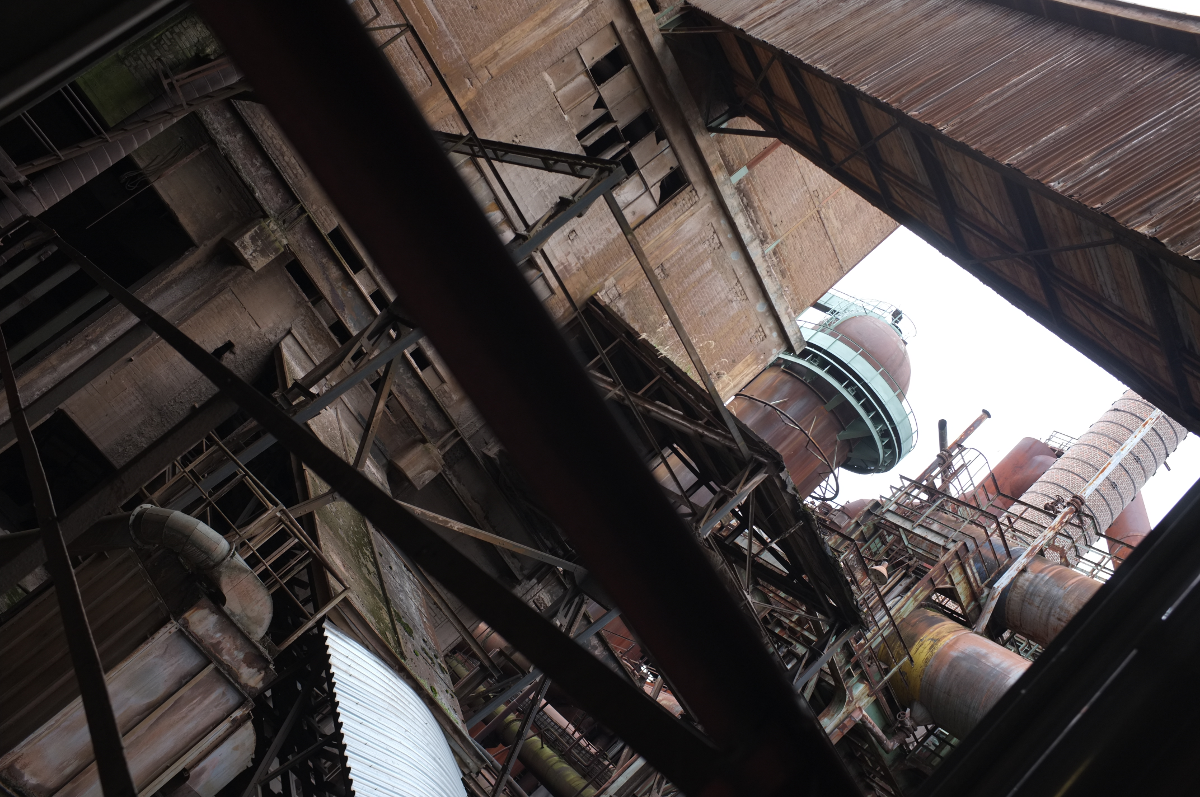
\includegraphics[width=0.7\textwidth]{Examples/example_5.png}
  \caption{Erstes Bild, Völklinger Hütte}
  \label{fig:Huette}
\end{figure}


\subsection{Wrapfigure}
Abbildung~\ref{fig:Huette} ist zwar ganz nett anzusehen, aber vielleicht sähe es eleganter aus, wenn die Abbildung 
von unserem Textabschnitt umflossen werden würde. Diese Art von Abbildungen sollte jedoch sparsam und mit großer Sorgfalt eingesetzt werden, da es zu unschönen Darstellungen kommen kann.
\blindtext
\begin{wrapfigure}{l}{0.4\textwidth}
  \centering
  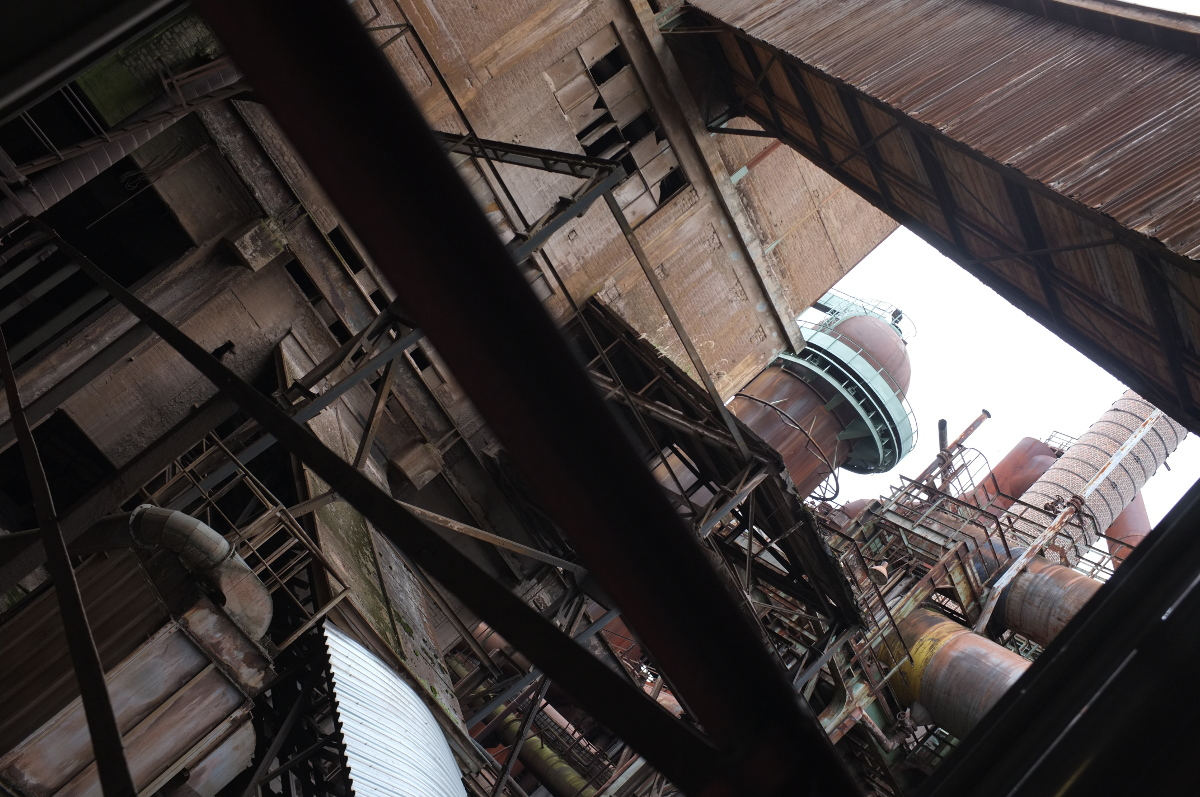
\includegraphics[width=0.4\textwidth]{Examples/example_5.jpg}
  \caption{Völklinger Hütte, *.jpg}
  \label{fig:Huette2}
\end{wrapfigure}
\blindtext


\subsection{Subfigures}
Es ist ebenso möglich, mehrere Abbildungen nebeneinander zu setzen, wie in Abbildung~\ref{fig:Beide} zu sehen ist. Eine separate Referenzierung ist auch möglich: Abbildung~\ref{subfig:abbone}.
\begin{figure}[bth]
  \subfloat[Erstes ...]{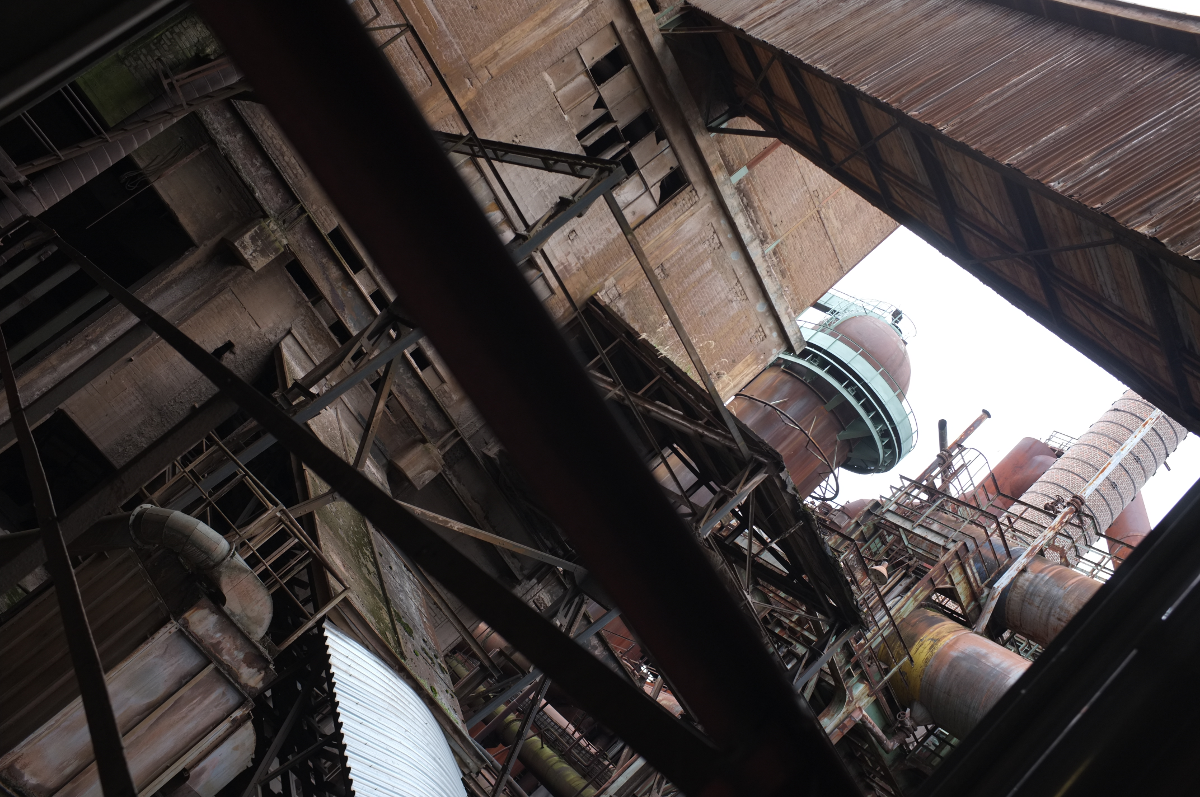
\includegraphics[width=0.49\textwidth]{Examples/example_5.png}\label{subfig:abbone}}\hfill
  \subfloat[... und zweites Bild]{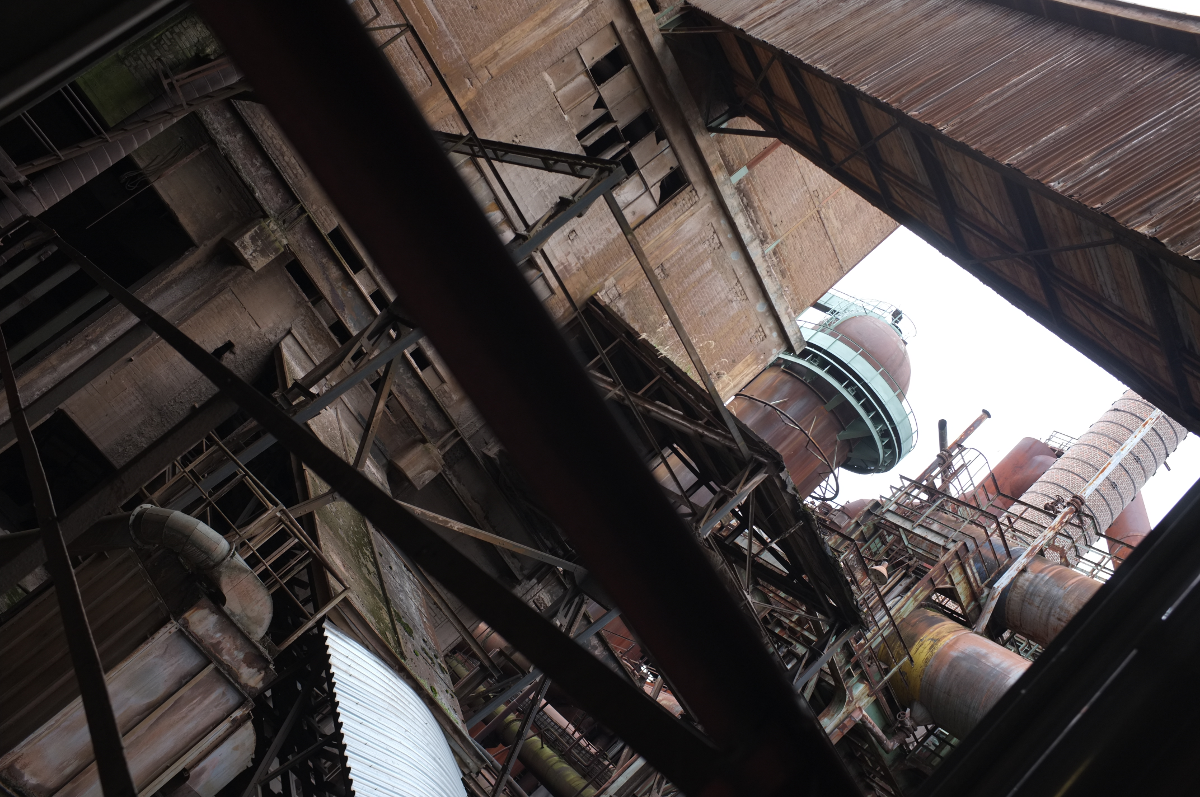
\includegraphics[width=0.49\textwidth]{Examples/example_5.png}\label{subfig:abbtwo}}
  \caption{Mehrere Abbildungen nebeneinander}
  \label{fig:Beide}
\end{figure}


\subsection{Qualitätsunterschiede}
\begin{figure}[p]
	\centering
  \subfloat[\textit{PDF}-Format]{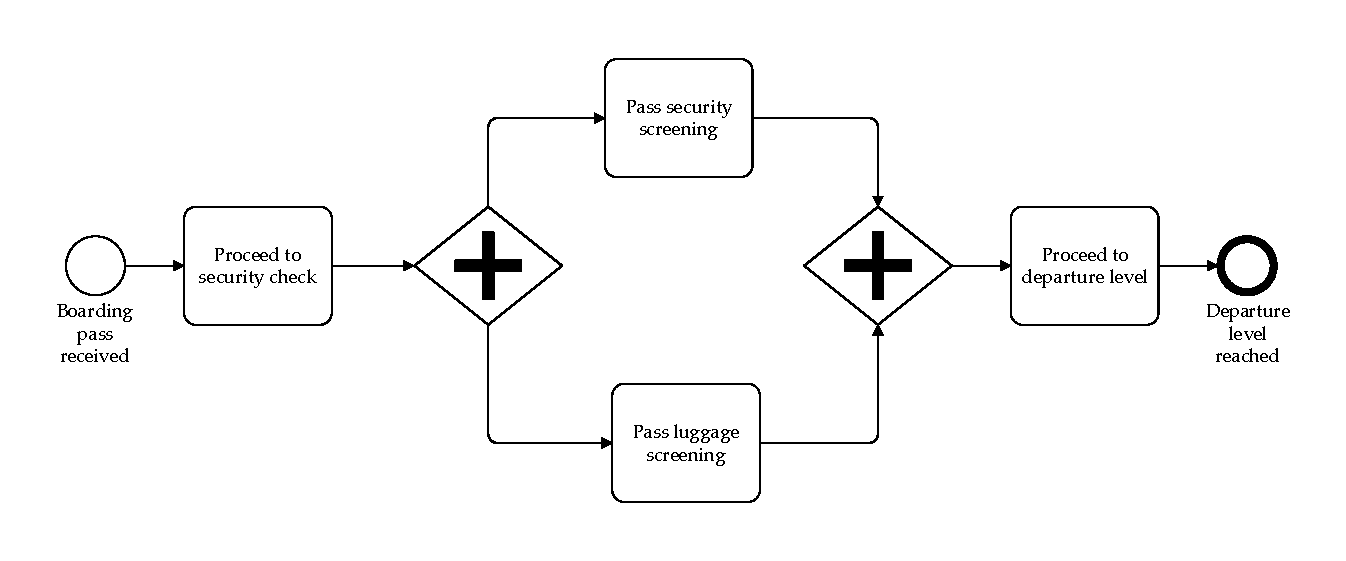
\includegraphics[width=0.65\textwidth]{Examples/bpmn.pdf}} \\
  \subfloat[\textit{JPG}-Format]{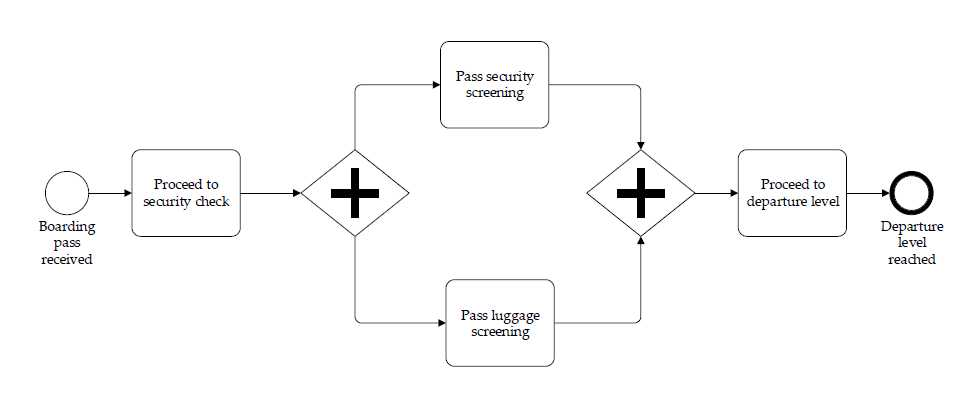
\includegraphics[width=0.65\textwidth]{Examples/bpmn.jpg}}
  \caption{Beide Formate im Vergleich}
  \label{fig:pdfvsjpg}
\end{figure}

\begin{figure}[p]
	\centering
  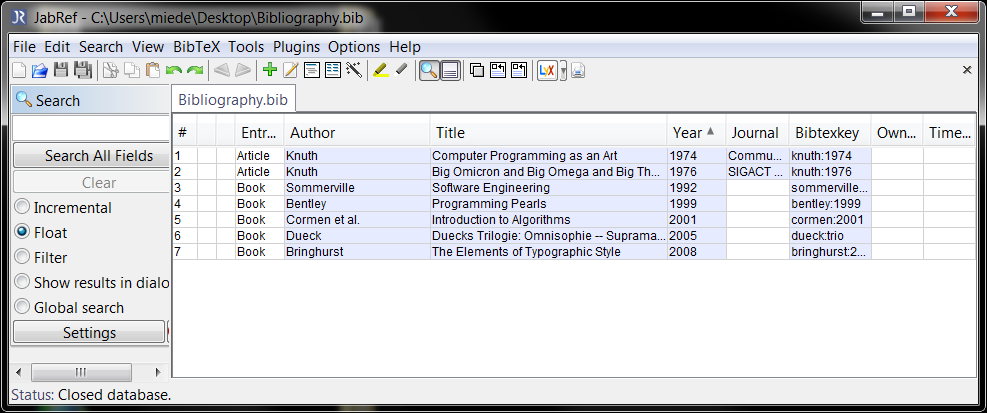
\includegraphics[width=0.65\textwidth]{Examples/jabref.png}
   \caption{\textit{PNG}-Format}
  \label{fig:pngvsjpg1}
\end{figure}

\begin{figure}[p]
	\centering
  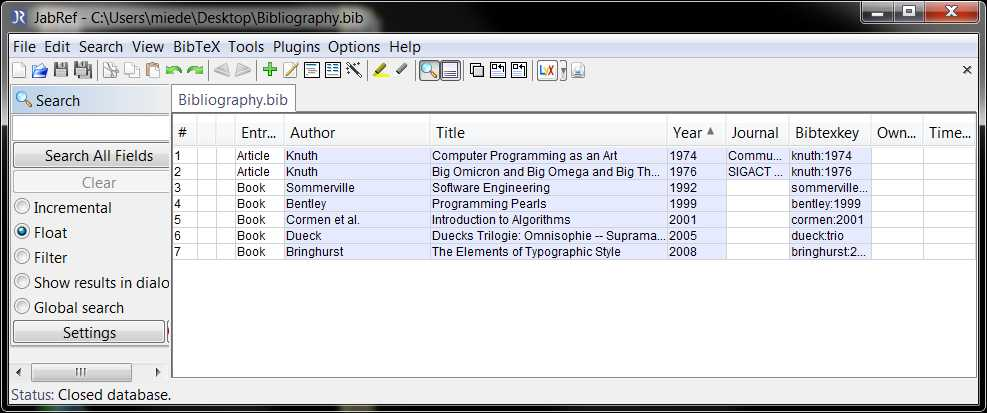
\includegraphics[width=0.65\textwidth]{Examples/jabref.jpg}
   \caption{\textit{JPG}-Format}
  \label{fig:pngvsjpg2}
\end{figure}

Leider haben die unterschiedlichen Grafikformate bedingt durch die unterschiedlichen Kompressionsverfahren einige Schwächen, insbesondere die Umwandlung in das \textit{JPG}-Format erzeugt unangenehme Artefakte im Bild. \autoref{fig:pdfvsjpg} zeigt die Unterschiede zwischen \textit{PDF-Format} und \textit{JPG-Format} im Vergleich. 

Wenn eine \textit{*.pdf}-Datei nicht infrage kommt, beispielsweise bei Screenshots, ist unbedingt das \textit{PNG-Format} vorzuziehen. 
Den Unterschied machen \autoref{fig:pngvsjpg1} und \autoref{fig:pngvsjpg2} deutlich.

\glqq Faustregeln\grqq im Umgang mit Abbildungen:
\begin{itemize}
	\item Diagramme bzw. alles, was Linien usw. enthält: \textit{PDF} (im Vektorformat).
	\item Screenshots bzw. alles, was größere gleichfarbige Flächen enthält: \textit{PNG}.
	\item Der Rest (in der Regel Fotos): \textit{JPEG}.
\end{itemize}





%*******************************
% 			Listings 		   *
%*******************************

\section{Quellcode einbinden}
Das Package \textit{lstlisting} ermöglicht es, Quellcode ansprechend in das Dokument einzubinden. Man kann Quellcode einzeilig einbinden 
mittels \lstinline{\lstinline|Quellcode|}. Dabei ist darauf zu achten, dass der Befehl einmal mit \{ \} und einmal mit | | aufgerufen werden kann, je nachdem, 
welche Zeichen im angegebenen Quelltext genutzt werden. 
Es ist auch möglich eine eigene Umgebung für Quelltext zu schaffen:

\begin{lstlisting}[caption=Erstes Listing,style=Java]
private Umgebung(int i, int k)
{
	System.out.println("Eine Funktion mit " + i + "und" + k ".");
}
\end{lstlisting}  

Wer Quelltext aus externen Dateien einbinden möchte, geht wie folgt vor:

\lstinputlisting
[caption={Externer Quellcode},style=Java]
{Examples/Code.java}

Wie genau der Quellcode formatiert und gefärbt ist, ist in \textit{htwsaar.i.mst.config.tex} hinterlegt, wobei fü verschiedene Sprachen auch eigene Styles angelegt werden
können (hier z.B. für Java).
\section{Mathematische Ausdrücke}
Mathematische Ausdrücke sind eine kleine Kunst für sich. Am allereinfachsten kann man eine Formel, wie \(a + b = c\) in den Fließtext einbinden, wobei LaTeX die Höhe der Ausdrücke der Zeile anpasst,
wie hier zu sehen \(\sum_{y=0}^{x} a\) . In einer Umgebung sieht das schon anders aus:
\begin{equation}
  \sum_{y=0}^{x} a
\end{equation}

Griechische Buchstaben:
\begin{equation}
	\alpha\beta\gamma\delta\epsilon\varepsilon\zeta\eta
	\theta\iota\kappa\lambda\mu\nu\xi\pi\varpi\rho\varrho
	\sigma\tau\upsilon\phi\varphi\chi\psi\omega
\end{equation}

Brüche:
\begin{equation}
	Ergebnis = \frac{a}{b}
\end{equation}

\begin{equation}
	\frac{\sin{\alpha}^2 + \cos{\alpha}^2}{1} = 1
\end{equation}

\begin{equation}
	\frac{-9x}{\frac{2y}{3z+2}}
\end{equation}

Text innerhalb von Formeln:
\begin{equation}
\sum_{y=1}^{n} y = \frac{n*(n+1)}{2}
\quad
\text{Gaußsche Summenformel}
\end{equation}

Hoch- bzw. Tiefstellungen:
\begin{equation}
	x_{i,j}^2
\end{equation}

\begin{equation}
	{x_{i,j}}^2
\end{equation}

\begin{equation}
	x_{n_0}
\end{equation}


Matrizen:
Matrizen werden innerhalb der mathematischen Umgebung als wiederum neue Umgebung eingebunden. Wie bei Tabellen auch werden Zeilen durch \lstinline{\\} und Spalten durch \lstinline{&} getrennt.

\begin{equation}
	\begin{pmatrix} 
		a&b\\
		c&d 
	\end{pmatrix}
\end{equation} 

\begin{equation}
	\begin{vmatrix} 
		a&b\\
		c&d 
	\end{vmatrix}
\end{equation} 

Fallunterscheidung:
\begin{equation}
	f(x) = 
	\begin{cases}
		0, &\text{falls } x < 0 \\
		1, &\text{falls } x \geq 0
	\end{cases}
\end{equation}




%############################################################
\clearpage\section{To-Do-Notes}
Um bei einer längeren Arbeit nicht den Überblick zu verlieren, an welcher Stelle es nötig ist
weiter zu arbeiten, bietet es sich an, kleine Notizen einzufügen. Das Package \textit{todonotes}
stellt eine elegante Lösung bereit, um differenziert und vielfarbig jene Abschnitte zu kennzeichnen,
die einer weiteren Bearbeitung bedürfen.

\subsection*{Beispiel für To-Do-Notes}
Dies hier ist ein Blindtext zum Testen von Textausgaben. Wer diesen Text liest, ist selbst
\todo{Plain todonotes.} schuld. Der Text gibt lediglich den Grauwert der Schrift an. Ist das wirklich so? Ist es
gleichgültig, ob ich schreibe: Dies ist ein Blindtext? oder Huardest gefburn? Kjift?
mitnichten! Ein Blindtext bietet mir wichtige Informationen. An ihm messe ich die Les-
barkeit einer Schrift, ihre Anmutung, \todo{Plain todonotes.}wie harmonisch die Figuren zueinander stehen
und prüfe, wie breit oder schmal sie läuft. Ein Blindtext sollte möglichst viele verschie-
dene Buchstaben enthalten und in der Originalsprache gesetzt sein. Er muss keinen
Sinn ergeben, sollte aber lesbar sein.\todo[nolist]{Todonote that is only shown in the margin and not in
the list of todos.}%
Fremdsprachige Texte wie Lorem ipsum dienen
nicht dem eigentlichen Zweck, da sie eine falsche Anmutung vermitteln. Dies hier ist
ein Blindtext zum Testen von Textausgaben. Wer diesen Text liest, ist selbst schuld. 

\todo[inline]{A very long todonote that certainly will fill more
than a single line in the list of todos. Just to make sure let's add
some more text \ldots}

Der Text gibt lediglich den Grauwert der Schrift an. Ist das wirklich so? Ist es gleichgültig,
ob ich schreibe: Dies ist ein Blindtext? oder Huardest gefburn? Kjift? mitnichten!
\todo[noline]{A note with no line back to the text.}
Ein Blindtext bietet mir wichtige Informationen. An ihm messe ich die Lesbarkeit einer
Schrift, ihre Anmutung, wie harmonisch die Figuren zueinander stehen und prüfe, wie
\todo[caption={A short entry in the list of todos}]{A very long
todonote that certainly will fill more than a single line in the
list of todos \ldots}
breit oder schmal sie läuft. Ein Blindtext sollte möglichst viele verschiedene Buchstaben
enthalten und in der Originalsprache gesetzt sein. Er muss keinen Sinn ergeben, sollte
aber lesbar sein. Fremdsprachige Texte wie Lorem ipsum dienen nicht dem eigentlichen Zweck, 
da sie eine falsche Anmutung vermitteln.
\missingfigure{A figure I have to make \ldots}

%Nummerierte ToDo-Notes
\todox{Erste Nummer...}
\todox{Zweite Nummer...}

%Alles To-Dos als Liste ausgegeben
Nachfolgend wird noch eine Liste aller To-Dos auf einer separaten 
Seite ausgegeben.
%\begingroup
	%\let\clearpage\relax
	%\let\cleardoublepage\relax
	\listoftodos
%\endgroup 


 		% Abschlussarbeit geht!



\chapter{Was sind Microservices?}\label{sec:microservices}

Prinzipiell ist es schwierig Microservices einheitlich zu definieren. Gründe dafür sind zum einen, dass das Prinzip von Microservice-Architekturen zwar klar ist, es aber dennoch unterschiedliche Ansichten und Verständnisse  diesbezüglich in der Fachliteratur gibt. Zum anderen gibt es keine einheitliche Architektur von Microservices, bzw. das Grundprinzip ist klar, dies wird allerdings unterschiedlich umgesetzt. Genaueres zu der uneinheitlichen Architektur von Microservices wird in \ref{sec:funktionsweise} beschrieben.\newline\newline 

„Eine Microservicearchitektur besteht aus einer Sammlung kleiner, autonomer Dienste. Jeder Dienst ist eigenständig und sollte eine einzige Geschäftsfunktion implementieren.“\cite{microsoft}\newline\newline 

„Die Microservice-Architektur - oder einfach nur Microservices - ist eine eigene Entwicklungsmethode für Softwaresysteme, die sich auf die Entwicklung von Modulen mit nur einer Funktion mit gut definierten Schnittstellen und Operation zu konzentrieren versucht.“\cite{smartbear}\newline\newline 

„A microservice, in my mind, is a small application that can be deployed independently, scaled independently, and tested independently and that has a single responsibility. It is a single responsibility in the original sense that it's got a single reason to change and/or a single reason to be replaced. But the other axis is a single responsibility in the sense that it does only one thing and one thing alone and can be easily understood.“\cite{ieeetalk}\newline\newline 

Man sieht, das es keine standardisierte, formalisierte Definition von Microservices gibt. Dennoch gibt es grundlegende charakteristische Merkmale die diese Architektur beschreiben.\newline
Microservices ist eine Methode zur Entwicklung von Softwareanwendungen als Umgebung von unabhängigen, voneinander einsetzbaren, modularen Diensten. Jeder Service soll so konfiguriert sein, das er als alleiniger Dienst ausgeführt werden kann, Daten unabhängig von anderen Diensten verarbeitet und nur über genau definierte Schnittstellen mit anderen Services kommuniziert.\cite{keyhole}\newline

Genauer gesagt Microservice ist ein Ansatz zur Modularisierung von Software. Das heißt große Software-Systeme sollen in kleine Module unterteilt und entwickelt werden.\newline
Dadurch soll es möglich sein Software einfacher zu erstellen, zu verstehen und weiterzuentwickeln. Des Weiteren sollen Microservices möglichst klein, unabhängig und lose gekoppelt sein. Ein Dienst wird von einem kleinen Entwicklerteam geschrieben und verwaltet. Microservices werden unabhängig von einander bereitgestellt, getestet und deployt.\newpage 

Das Konzept des Microservice verfolgt den gleichen Ansatz wie die Unix-Philosophie\cite{unixphilosophie}\newline
\begin{description}
 \item - Ein Programm soll genau eine Aufgabe erledigen. Diese soll aber richtig erledigt werden.
 \item - Programme sollen zusammen arbeiten können.
 \item - Es sollen universelle Schnittstellen genutzt werden.
\end{description}


\chapter{Wie funktionieren Microservices?}\label{sec:funktionsweise}

Wie schon im vorherigen Abschnitt erwähnt sind Microservices modular aufgebaut und sollen nur über geeignete Schnittstellen miteinander/mit dem Programm kommunizieren. Daher wird jeder Microservice auf einem eigenen Server betrieben, wobei die Services voneinander nichts wissen sollen. Die Funktionsweise bzw. der genaue Ablauf eines Microservices wird in \ref{sec:funktion} beschrieben.\newline\newline

\begin{figure}[bth]
    \centering
    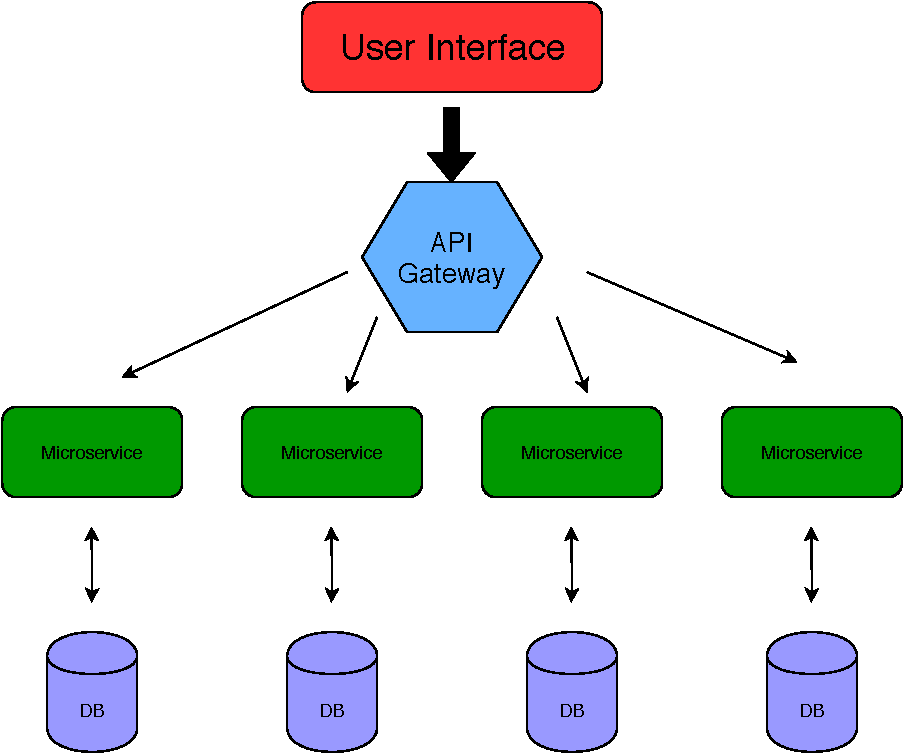
\includegraphics[width=0.8\textwidth]{Chapters/Bilder/Microservices.pdf}
    \caption{Microservice}
   \label{fig:microservice}
  \end{figure}
  
\newpage

\ref{fig:microservice} zeigt einen grundlegenden Aufbau eines Microservices. Wie im vorherigen Abschnitt erwähnt ist es schwierig eine einheitliche Architektur für Microservices zu definieren. Dies wird im folgenden Abschnitt beschrieben.
Wie man dennoch zu einer guten Architektur kommt, die auf die Organisation und oder das Programm passt und welche Herausforderungen dabei beachtet und bewältigt werden müssen wird in \ref{ch:Herausforderungen} beschrieben.\newline\newline

Vom Grundgedanken her besitzt jeder Microservice sein eigenes User Interface, durch welches der Nutzer mit der Software kommunizieren soll. Da Microservices allerdings modular aufgebaut sind und im besten Fall unabhängig von einander sind müssen die einzelnen User Interfaces der Microservices noch einmal in einer großen Master IU zusammen gefasst werden. Diese Master UI dient dazu, die einzelnen User Interfaces der Microservices zu bündeln und dem Nutzer so eine UI zur Verfügung zu stellen, sodass es den anschien hat das es eine einzige UI ist. Dieser Architektur-Ansatz wird allerdings eher selten in der Praxis genutzt, da es ohne ausreichender Kommunikation unter den Teams bzw. ohne eines grundlegenden Designs der Oberfläche zu Inkonsistenz und unterschiedlich aussehenden Bausteinen der UI kommen kann.
Daher wird bei der Erstellung von Microservices eher auf den Aufbau wie in \ref{fig:microservice} zurückgegriffen, d.h es gibt ein gemeinsames User Interface das von einem Team erstellt und verwaltet wird. Dadurch entsteht zwar im Umkehrschluss eine erhöhte Kommunikation der einzelnen Microservice Teams und des UI Teams, wenn neue Features implementiert werden müssen. Allerdings ist auf der anderen Seite eine einheitliche und runde Oberfläche gewährleistet. Dies ist gerade für den Endnutzer von Vorteil, da er dadurch ein angenehmeres Gefühl bei der Arbeit mit der Software hat.\newline\newline

Wie am Anfang des Abschnitts beschrieben liegt jeder Microservice auf einem eigenen Server und kann nur über eine Schnittstelle nach außen kommunizieren. An dieser Stelle kommt das API-Gateway ins Spiel.
Das API-Gateway dient als Einstiegspunk für die Clients. Das bedeutet anstatt den Service direkt aufzurufen, rufen die Clients das API-Gateway auf. Dieses leitet anschließend den Aufruf an den geeigneten Service im Back-End weiter.  Dies hat unter anderem die Vorteile, dass\cite{microsoft}:
\begin{description}
	\item - Es entkoppelt die Clients von den Diensten. Für Dienste kann eine Versionierung oder Umgestaltung durchgeführt werden, ohne dass sämtliche Clients aktualisiert werden müssen. 
	\item - Dienste können nicht web fähige Messagingprotokolle verwenden, z.B. AMQP. (Was ist das)
	\item - Das API-Gateway kann weitere übergreifende Funktionen ausführen, beispielsweise Authentifizierung, Protokollierung, SSL-Terminierung und Lastenausgleich.
\end{description}

Allerdings ist das API-Gateway kein Muss bei der Implementierung einer Microserice-Architektur sondern eine Möglichkeit seine Architektur übersichtlicher zu gestalten. Gerade bei kleineren Software-Systemen kann man auf ein API-Gateway verzichten und die Kommunikation zwischen UI und Microservice über Frameworks wie zum Beispiel REST gestalten. Diese Art der Kommunikation wird auch im Kapitel \ref{ch:Fallstudie} genutzt, um zu zeigen wie solch eine Architektur in einem System funktionieren kann.\newpage


Jeder Microservice hat seine eigenes Back-End in dem die Bussines-Logic enthalten ist. Dort wird genau eine Funktionalität implementiert und es soll möglichst darauf geachtet werden das kein Service von anderen Services abhängig ist geschweige denn Funktionalitäten von anderen Services enthält. Auf dieses Problem wird noch einmal genauer in Kapitel \ref{ch:Herausforderungen} eingegangen, wie damit umzugehen ist.\newline\newline

Prinzipiell hat jeder Microservices seine eigene Datenhaltungsschicht auf die nur er zugreifen kann/soll. Allerdings gibt es auch Ansätze bei denen sich mehrere Microservices eine gemeinsame Datenhaltung teilen bzw. auf mehrere Datenhaltungen zugreifen. Dieser Ansatz wird auch in \ref{ch:Fallstudie} genutzt. 
Welche Art der Datenhaltung genutzt wird, sollte Projekt und Architekt abhängig betrachtet werden, da es bei Zugriffen von mehreren Services auf dieselbe Datenhaltung schnell zu Problemen kommen kann. Welche Probleme an dieser Stelle genau auftreten können und wie diese zu lösen sind wird genauer in \ref{ch:Daten} beschrieben.

\section{Funktionsweise}\label{sec:funktion}

Ein Client nutzt die Software welche aus einer Microservice-Architektur besteht. Über das User-Interface kann er mit dem System kommunizieren. Möchte er nun eine Funktionalität der Software nutzen, wird zuerst die Anfrage an das API-Gateway geleitet. Dieses schaut welche Microservices für diese Anfrage zuständig sind und leitet anschließend die Anfrage an den/die entsprechenden Services weiter. Diese bearbeiten die Anfrage und geben das Ergebnis zurück an das API-Gateway sodass das Ergebnis nun auf der UI dargestellt werden kann. Die genaue Kommunikation kann zum Beispiel über eine REST-Schnittstelle laufen welche JSON-Objekte empfängt und versendet.

\chapter{Vergleich mit anderen Architektur-Stilen}

In diesem Abschnitt beschäftigen wir uns mit dem Vergleich der Microservice-Architektur gegenüber dem herkömmlichen Architektur-Stil des Monolithen, sowie der ähnlich aufgebauten Architektur der Service Oriented Architecture. Kurz SOA.
Dabei wird zuerst darauf geschaut was sich hinter diesen beiden Architektur-Stilen verbirgt und wie diese funktionieren. Anschließend wird ein Vergleich zwischen dem Microservices und der jeweiligen Architektur gezogen.

\section{Vergleich Monolith}

Um zu schauen in wie fern sich die Architektur eines Microservice mit der Architektur eines Monolithen unterscheidet, muss zuerst geklärt werden was unter einem Monolithen verstanden wird.\newline\newline

Ein Monolith ist ein Software-System welches als eine große untrennbare Einheit gestaltet wird. Die monolithische Architektur folgt keiner expliziten Gliederung in Teilsysteme sondern wird als ein ganzes Software-System betrachtet.\cite{monolith}
Dieses Software-System, häufig auch als Legacy-System bezeichnet, besteht im Endeffekt aus einer  einzelnen logisch ausführbaren Datei. Diese beinhaltet die gesamte Logik der Software und wird serverseitig verwaltet. Die Software läuft meist in einem einzigen Prozess auf einem Server, auf den von außerhalb zugegriffen werden kann. 
Da es sich bei dem Monolithen um eine ausführbare Datei handelt, muss bei jeder Änderung an dem System der Aufbau und die Bereitstellung einer neuen Version, für die serverseitige Anwendung gewährleistet sein.\cite{fowlerlewis}

\begin{figure}[bth]
    \centering
    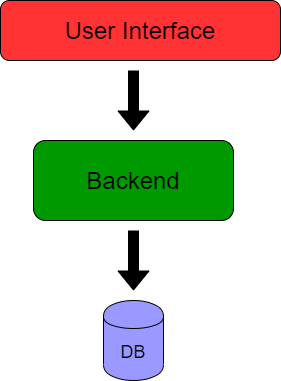
\includegraphics[width=0.4\textwidth]{Chapters/Bilder/Monolith.png}
    \caption{Monolith}
   \label{fig:monolith}
  \end{figure}
  
\ref{fig:monolith} zeigt den prinzipiellen Aufbau und die Funktionsweise eines Monolithen.
Dieser ist in drei Schichten aufgeteilt: dem User Interface, der Backend und der Datenhaltungsschicht.
Das User Interface bietet die Möglichkeit der Kommunikation mit dem System. Es empfängt Ereignisse und leitet diese an das Backend weiter.
Im Backend befindet sich die gesamte Business-Logik des Software-Systems. Es verarbeitet die empfangenen Nachrichten und greift auf die entsprechend benötigten Daten in der Datenhalten zu.
Die Datenhaltungsschicht beinhaltet alle benötigten Daten die das Software-System verarbeitet.\newline\newline

Vergleicht man nun die Architektur des Microservices mit der Architektur des Monolithen gibt es auf der einen Seite Ähnlichkeiten in Bezug auf die einzelnen Komponenten.\newline
Man könnte sagen das jeder Microservice ein sehr kleiner Monolith sei, da jeder Microservice je nach Architektur sein eigenes User Interface besitzt. Ein eigenes Backend sowie eine eigene Datenhaltung hat. Dies steht aber im Widerspruch mit der Bedeutung eines Monolithen, bei dem es sich um eine große Einheit handelt und ein Microservice meist nur aus wenigen Funktionalitäten. Dennoch ist der Vergleich naheliegend.\newline
Im Vergleich zu dem Monolithen liegen die einzelnen Microservices auf unterschiedlichen Servern, wodurch die Kommunikation über spezielle Schnittstellen umgesetzt wird, welche über das Internet miteinander kommunizieren. Bei einem Monolithen ist dies nicht der Fall, da die gesamten Funktionalitäten auf einem Server liegen und dadurch direkt aufgerufen werden können. Auch die Datenhaltung unterscheidet sich bei einem Microservice und dem Monolithen, da jeder Microservice meist seine eigene Datenhaltung besitzt und ein Monolith meist nur auf eine oder wenige Datenhaltungen zugreift.\newline
Ein wesentlicher Unterschied zwischen den beiden Architektur-Stilen ist der Umgang mit Abhängigkeiten. Da jeder Microservice auf einem eigenen Server läuft und nur für einen einzige Funktionalität zuständig ist, ist es wichtig das wenige, im Idealfall, keine Abhängigkeiten zwischen Microservices entstehen, da dies zu erheblichen Problemen führen kann. Genaueres zu dieser Problematik in Kapitel \ref{ch:Herausforderungen}.\newline
Bei einem Monolithen sollte zwar auch Wert auf eine saubere Architektur gelegt werden und dadurch sehr genau auf Abhängigkeiten geachtet werden. Dennoch ist es an dieser Stelle nicht so gravierend bzw. Abhängigkeiten werden sogar benötigt. 
Ein weiterer Unterschied ist die Aufteilung der Entwicklerteams. Bei einem Monolithen werden die Teams auf der technischen Ebene aufgeteilt. Das heißt, ein Team ist für die Datenhaltung zuständig, ein anderes Team kümmert sich um die Business-Logik und ein weiteres Team ist für die graphische Oberfläche verantwortlich.\newline
Bei einem Microservices werden die Teams nach Fachlichkeit des Geschäftsprozesses aufgeteilt. \newline
Hier ist ein Team zum Beispiel für die Artikelsuche eines Online-Shops zuständig. Ein weiteres für den Warenkorb und ein drittes Team für den Kaufabschluss. Dadurch ist jedes Team für einen Geschäftsprozess alleine verantwortlich und muss sich sowohl um die Nutzeroberfläche als auch um die Business-Logik und die Datenhaltung kümmern.\newpage


\section{Vergleich SOA}

Schaut man sich die beiden Architektur-Stile Microservice und SOA an, scheinen sie auf dem ersten Blick recht identisch zu sein. Bei beiden Ansätzen steht die Aufteilung großer Systeme in kleinere Services im Vordergrund. Daher werden in der Literatur Microservices und SOA häufig als dasselbe bezeichnet, da sich beide Ansätze mit der Aufteilung von Anwendungen in Services beschäftigen. Schaut man sich die beiden Ansätze nun aber genauer an stellt man fest, das sie sich in bestimmten Punkten weit aus mehr unterscheiden als zuvor angenommen.\cite{microservices}

Für Service Oriented Architecture oder kurz SOA  gibt es, wie für Microservices, keine einheitliche Definition. Dennoch gibt es zentrale Bestandteile dieser Architektur, welche große Ähnlichkeiten mit Microservices aufweisen. 
Unter anderem besteht SOA wie Microservices aus Services welche eine Funktionalität umfassen sollen, sowie das der Service eigenständig genutzt werden kann. Des weiteren sollen die Services über das Internet und über eine geeignete Schnittstelle miteinander kommunizieren. Auch ist die Nutzung von verschiedenen Programmiersprachen sowie Frameworks bei der Entwicklung von SOA möglich.\cite{microservices}\cite{soa}

\begin{figure}[bth]
    \centering
    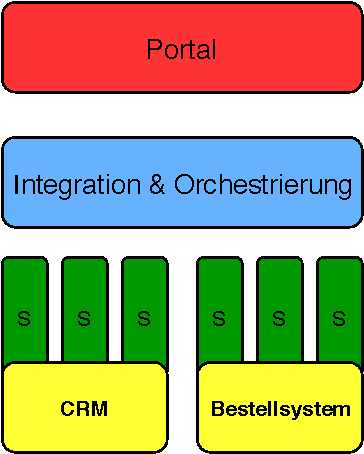
\includegraphics[width=0.4\textwidth]{Chapters/Bilder/SOA.pdf}
    \caption{SOA}
   \label{fig:soa}
  \end{figure}
  
\ref{fig:soa} zeigt einen möglichen Architekturansatz und die Funktionsweise eines SOA-Systems. SOA besteht aus einem Portal, einer Integrations- und Orchestrierungsschicht sowie aus mehreren größeren Services welche zu einer bestimmten Fachlichkeit des Geschäftsprozesses gehören. Jeder Service besteht noch einmal aus mehreren kleineren Services.\newline
Das Portal ist vergleichbar bzw. das gleiche wie ein User Interface welches bei den beiden anderen Ansätzen zum Einsatz kommt. Es ist dafür zuständig, Nutzern eine Oberfläche zu bieten, mit der die Services verwendet werden können. Es können auch mehrere Portale koexistieren, jeweils für unterschiedliche Nutzer des Systems. Zum Beispiel für Kunden, den eigenen Support oder auch interne Mitarbeiter wie Verwaltung oder Management. Aber auch für unterschiedliche Plattformen wie Desktop oder mobile Apps. Egal welche Art von Portal, für die Architektur macht dies keinen Unterschied.\newline
In der Integrations- \& Orchestrierungsschicht sind die einzelnen Services in einem Verzeichnis registriert. Sie übernehmen die Anfragen der Clients, suchen nach den entsprechenden Services die für dies Anfrage benötigt werden und rufen diese mit den entsprechenden Daten auf.\newline
Die größeren Services sind wie schon erwähnt in Fachlichkeiten des Geschäftsprozesses unterteilt und beinhalten wiederum mehrere kleinere Services, vergleichbar mit Microservices, welche zu Umsetzung einzelner kleinere Geschäftsprozesse dienen. Als Beispiel beinhaltet ein Service das Customer Relationship Management (CRM), welches sich um die Kundenverwaltung kümmert. Die einzelnen Services sind dann für die einzelnen Prozesse des CRM zuständig wie zum Beispiel, Kunde registrieren, Kunde löschen oder Kunde ändern. Jeder größere Service beinhaltet eine eigene Datenhaltung, auf die, die einzelnen Services zugreifen können.\newline\newline

Vergleicht man nun beide Ansätze stellt man fest, das es wie schon erwähnt viele Gemeinsamkeiten gibt, aber auch große Unterscheide, wodurch es schwierig wird Microservices und SOA als das gleiche zu betrachten.\newline
Beide Ansätze streben die Aufteilung von Anwendungen in Services an, sowie die Kommunikation der einzelnen Services über das Netzwerk.\newline
Aber schon bei der Kommunikation bzw. der Integration fangen die Unterschiede an. Bei SOA funktioniert die Integration auch für Orchestrierung. An dieser Stelle wird ein Geschäftsprozess aus den einzelnen Services zusammengesetzt. Die Orchestrierung soll so eine gewisse Flexibilität in das Programm bringen. Bei Microservices hat die Integrationslösung keine eigene Intelligenz. Die einzelnen Services kommunizieren untereinander und müssen sich kennen. Microservices versuchen hingegen die Flexibilität durch einfache und schnelle Änderung sowie Ersetzung von Services zu gewährleisten.\newline
Ein weiterer Unterschied ist die Aufteilung der Teams in Fachlichkeit und Technik.
Bei SOA gibt es ein Team welches für die Oberfläche bzw. das Portal zuständig ist. Ein Team welches sich um die Integration \& Orchestrierung kümmert. Diese beiden Teams sind auf technische Weise aufgeteilt. Andere Teams kümmern sich um die einzelnen fachlichen Aspekte des Systems, wobei diese für eine Sammlung von Services des jeweiligen Geschäftsprozesses zuständig sind. Durch die Integration und Orchestrierung muss eine unternehmensweite Integrationslösung eingeführt werden, da es gerade bei dem Zugriff auf Daten zu Problemen führen kann. Bei Microservices ist dies leichter zu handhaben, da es keine einheitliche Integrationstechnologie gibt. Die Technologie der Integration und Kommunikation ist auf den Service begrenzt. Gerade bei Datenreplikationen ist dies von Vorteil. Genaueres hierzu in \ref{ch:Daten}.\newline
Auch die Kommunikation zwischen mehreren Teams ist bei SAO schwieriger als bei Microservices. Durch die Aufteilung auf technischer Ebene kann es bei Änderungen eines Service dazuführen, das Anpassungen an anderer Stelle, für die ein anderes Team verantwortlich ist, getätigt werden müssen. So muss zum Beispiel bei der Änderung eines Services auch die Oberfläche entsprechend geändert werden, wodurch das Team Service mit dem Team Portal kommunizieren muss.\cite{microservices}

\chapter{Warum nutzt man Microservices?}

In diesem Abschnitt wird darüber gesprochen, wieso es sinnvoll ist eine Microservice-Architektur zu verwenden und welche spezifischen Vorteile solch ein Architektur Ansatz mit sich bringt.
In den vorherigen Abschnitten wurde bereits ein Teil der Vorteile leicht angeschnitten. Nun werden diese detaillierter dargestellt.
Da es sich bei den Vorteilen nicht nur um technische Aspekte handelt, werden diese in drei Kategorien unterteilt:
\begin{description}
	\item - Technische Vorteile
	\item - Organisatorische Vorteile
	\item - Geschäftliche Vorteile
\end{description}

\section{Technische Vorteile}

Wie schon in den vorherigen Abschnitten erwähnt sind Microservices modular aufgebaut und jeder Service liegt auf einem eigenen Server. Dadurch entsteht eine verteilte Kommunikationsstruktur. Diese ermöglicht es einem Service, mit anderen Services zu kommunizieren bzw. diese aufzurufen. Diese Kommunikationsinfrastruktur muss dementsprechende Möglichkeiten enthalten um die Kommunikation zwischen den Services zu ermöglichen. Ein Entwickler muss diese Infrastruktur genau beschreiben. Dadurch ist es schwieriger das Abhängigkeiten zwischen zwei oder mehreren Services entstehen, da der Entwickler diese explizit einbauen muss, um die Kommunikation zu gewährleisten. Falls sich doch einmal solch eine Abhängigkeit ungewollt einschleichen sollte, gibt es  spezielle Architekturmanagement-Werkzeuge um diese zu finden. Gerade bei Microservices ist dies leicht zu korrigieren, wenn man die Abhängigkeit frühzeitig entdeckt, da der Service schnell abgeändert werden kann oder komplett neu geschrieben werden kann. Genaueres zu dem Umgang mit Abhängigkeiten wird im Kapitel \ref{ch:Herausforderugen} beschrieben.\cite{microservices}\newline\newline

Ein weiterer Vorteil ist wie gerade beschrieben, die mögliche Ersetzung eines Microservices.
Gerade der Umgang mit alten Software-Systemen ist eine große Herausforderung. Oftmals ist die Codequalität recht schlecht, da die Software über Jahre hinweg von unterschiedlichen Entwicklern weiter entwickelt wurde und an vielen Stellen Hilfen eingebaut wurden, um temporäre Probleme zu lösen, die der Entwickler später wieder beheben wollte, dies aber nie tat. Diese Software weiter zu entwickeln oder gar neu zu schreiben ist ein fast unmögliches Unterfangen, da an vielen Stellen gar nicht mehr bekannt ist was einzelne Funktionen oder Codeabschnitte genau machen und der Entwickler der sie geschrieben hat, nicht mehr in dem Unternehmen tätig ist. Je größer die Software ist, desto größer ist der Aufwand. Beinhaltet die Software zusätzlich noch wichtige Geschäftsprozesse ist es praktisch unmöglich die Software noch zu ändern, da ein Ausfall der Software einen erheblichen finanziellen Schaden bedeuten kann.\newline
Microservices bieten an dieser Stelle den Vorteil das die Entwickler zum einen nicht an bestimmte Technologien gebunden sind, sondern können beliebige andere Technologien nutzen um das Problem zu lösen. Dadurch das ein Microservice im Idealfall auf der fachlichen Ebene eigenständig agiert, muss nicht genau bekannt sein wie die einzelnen Funktionen genau funktionieren. Dem Entwickler muss nur bekannt sein welche fachlichen Funktionalitäten der Microservices haben soll und welche Geschäftsprozesse er beinhaltet. Danach kann er diesen einfach durch einen neuen Microservice ersetzten.\cite{microservices}\newline\newline

Im Umgang mit Legacy-Systemen bilden Microservices einen weiteren Vorteil. Wie bei dem Vorteil der Ersetzung eines Microservices beschrieben, sind Legacy-Systeme oft recht unübersichtlich je größer sie werden. Mit Hilfe von Microservices können einzelne Codeabschnitte oder Funktionalitäten der Software einfach an einen Microservice ausgelagert werden. Hierzu muss einfach eine Schnittstelle an die Stelle der Funktionalität gebaut werden, welche ersetzt werden soll. Diese leitet die Anfrage anschließend an den Microservice weiter der diese dann verarbeitet. Anschließend kann er das Ergebnis wieder an das Legacy-System zurück senden, welches wiederum mit dem Ergebnis weiter arbeiten kann. Dadurch können kritische, schwer zu ändernde Codeabschnitte gezielt umgangen und ausgelagert werden, ohne das es zu Problemen mit dem System kommt.\cite{microservices}\newline\newline

Continous Delivery brint Software durch einen einfachen reproduzierbaren Prozess regelmäßig in Produktion. Dazu dient eine Continuous-Delivery-Pipeline.

\begin{figure}[bth]
    \centering
    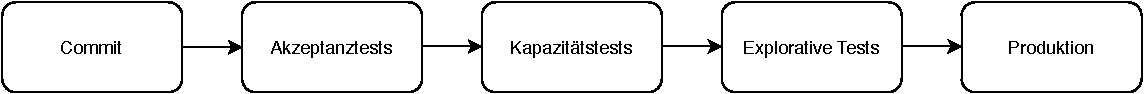
\includegraphics[width=1.0\textwidth]{Chapters/Bilder/CDP.pdf}
    \caption{Continuous-Delivery-Pipeline}
   \label{fig:cdp}
  \end{figure}

\begin{description}
	\item - In der Commit-Phase wird die Software kompiliert, die Unit-Tests werden durchgeführt und es wird gegebenenfalls eine statische Code-Analyse durchgeführt.
	\item - Die automatisierten Akzeptanztests in der nächsten Phase stellen sicher, dass die Software fachlich korrekt ist, sodass sie vom Kunden akzeptiert wird.
	\item - Kapazitätstests überprüfen, ob die Software performant genug ist, um die erwartete Anzahl Nutzer zu unterstützen. Auch diese Tests sind automatisiert.
	\item - Die explorativen Tests hingegen sind manuell und dienen dazu, bestimmte Bereiche des Systems zu testen. Dazu können neue Features zählen oder bestimmte Aspekte wie die Sicherheit des Systems.
	\item - Zum Schluss wird die Software in Produktion gebracht. Auch dieser Prozess ist idealerweise automatisiert.
\end{description}
\newpage
Die Software durchläuft jede einzelne Phase der CDP. Nach jeder erfolgreich abgeschlossenen Phase wird sie in der nächsten Phase weiter getestet. An dieser Stelle kann es passieren, dass die Software eine Phase erfolgreich abschließt, dann aber in der nächsten Phase nicht akzeptiert wird, weil zum Beispiel die Laufzeit zu lange dauert.\newline
Gerade hier liegt der Vorteil bei einer Microservice-Architektur. Microservices sind eigenständige Deployment-Einheiten. Daher können sie unabhängig von anderen Services getestet und in Produktion gebracht werden. Dies hat erhebliche Auswirkungen auf die CDP im Vergleich zum Testen von monolithischen Strukturen.
Der Durchlauf durch die einzelnen Tests ist wesentlich schneller, da nur ein kleiner Microservices in Produktion gebracht wird. Dadurch erhält man schnell Feedback, wodurch der Fehler bzw. das Problem behoben werden kann und sofort wieder getestet wird. Dadurch wird eine Menge zeit gespart. Denn wenn der Entwickler erst nach mehreren Tagen oder Wochen erfährt das sein Code fehlerhaft ist, ist es schwieriger sich wieder in den Code einzuarbeiten und den Fehler zu beheben.\newline
Auch ist der zu testende Aufwand wesentlich bei einem Microservice geringer als bei einem Monolithen. Bei einem Monolithen muss der gesamte Code bei einer Änderung wieder deployed und anschließen ausgeliefert werden. Bei einem Microservice ist es nur der Microservice selbst, ohne das andere Teiler der Software getestet und ausgeliefert werden müssen.\cite{microservices}\newline\newline

Auch in Bezug auf Skalierbarkeit haben Microservices Vorteile. Dadurch das jeder Service auf einem eigenen Server betrieben wird, können mehrere Instanzen des selben Microservice betrieben werden. Das heißt es gibt mehrere Services eines Microservices auf verschieden Servern. Dadurch ist eine gute Skalierbarkeit gewährleistet, da die Last auf mehrere Server verteilt werden kann. Auch ist es dadurch möglich Microservices auf unterschiedlich schnellen Servern laufen zu lassen. So kann jeder Microservice seine eigene Skalierung beinhalten. Des weiteren können so Microservices an verschiedenen Stellen im Netzwerk betrieben werden, um so einen geographische Skalierung zu erzeugen.\newline 
An dieser Stelle kommt auch die Robustheit eines Microservices in Spiel. Prinzipiell sollten Microservices anfälliger für Ausfälle sein, da ein Ausfall nicht nur auf der Hardware-Ebene passieren kann, sondern auch ein Ausfall auf der Netzwerk-Ebene. Um trotzdem eine hohe Verfügbarkeit zu gewährleisten muss eine Art Firewall zwischen den Microservices gebildet werden. Ein Ausfall eines Services darf sich nicht auf andere Services ausbreiten und diese ebenfalls zu einem Ausfall bringen. Hierzu kann zum einen bei einem Ausfall ein Microservice mit einem Default-Wert weiter arbeiten oder an einen anderweitig reduzierten Services weiter geleitet werden. Zum anderen kann wie bei Skalierbarkeit beschrieben, bei einem Ausfall eines Microservices einfach ein anderer Service eingesetzt werden, der die gleicher Funktionalität besitzt. Dies wird solange betrieben bis der ursprüngliche Services wieder verfügbar ist.\cite{microservices}\newline\newline

Wie schon in vorherigen Abschnitten beschrieben herrscht bei Microservices eine Technologiefreiheit. Jeder Services kann in einer anderen Programmiersprache geschrieben sein, mit unterschiedlichen Frameworks zusammen arbeiten oder aber auch an bestehende Sprachen angepasst werden. Dies bietet zum einen den Vorteil, das Funktionalitäten mit bestimmten Anforderungen in dafür geeigneten Sprachen geschrieben werden können. Nehmen wir an es wird viel Wert auf die Laufzeit gelegt, so kann der Service in C oder C++ geschrieben werden. Des weiteren ist es so möglich, leichter Microservices zu ersetzen, da man den Service nicht in der ursprünglichen Sprache ersetzten muss, sondern eine beliebige wählen kann. Falls zum Beispiel ein Service in Python geschrieben wurde und der Entwickler die Firma verlassen hat, kann der Service in einer anderen Sprache neu geschrieben werden, falls sich niemand mit Python auskennen sollte. So kann einiges an Einarbeitungszeit gespart werden. Auch die Arbeitsmoral und Motivation kann dadurch gesteigert werden. Durch die technologische Wahlfreiheit können neue Frameworks oder Sprachen getestet werden, ob diese für das Unternehmen lukrativ sind bzw. ob man diese auch in Zukunft für andere Projekte nutzen kann.\newline Normalerweise würde in einem Unternehmen die Zeit fehlen, das sich Entwickler in neue Technologien einarbeiten können, um zuschauen welchen Mehrwert diese für die Firma haben. Des weiteren sorgt die Möglichkeit der Wahlfreiheit für eine gewisse Abwechslung für die Entwickler. Diese müssen nicht Tag für Tag mit der selben Sprachen etc. arbeiten, sondern können sich auch mit neuen Technologien beschäftigen. Dadurch kann zumindest teilweise ein gewisser Trott vermieden werden und die Mitarbeiter neue Impulse setzten.\cite{microsoft}


\section{Organisatorische Vorteile}

Durch die technische Unabhängigkeit kann ein Team, welches für einen Microservice voll zuständig ist, die Unabhängigkeit komplett ausnutzen. Dadurch wird vor allem die Selbstständigkeit des Teams gestärkt. Des weiteren müssen die einzelnen Teams weniger koordiniert werden, da es zum Beispiel nicht wichtig ist das unterschiedliche Bibliotheken oder unterschiedliche Versionen von Bibliotheken genutzt werden.
Die einzelnen Teams sind dafür verantwortlich welche Architektur welche Sprache und weiches Framework genutzt wird. Daraus folgt aber auch, dass das Team die vollen Konsequenzen tragen muss, falls etwas schief läuft. Dies steigert zum einen die Selbstorganisation und zum anderen werden die Teammitglieder zusätzlich motiviert fokussiert zu arbeiten und ihre Entscheidungen zu reflektieren.\cite{microservices}

\section{Geschäftliche Vorteile}

Die bereits erwähnten Vorteile aus der organisatorischen Sicht führen zu geschäftlichen Vorteilen. Das Risiko der Projekte sinkt, da jedes Team eine hohe Eigenverantwortlichkeit trägt und die Koordinierung zwischen den Teams wird weniger, sodass die Teams effizienter arbeiten können.
Durch die Aufteilung in Mikroservices können die Teams unabhängig von einander an den Services Arbeiten, was eine parallele Arbeit ermöglicht. Teams müssen nicht auf Ergebnisse anderer Teams warten , um selbst an ihren Services weiter arbeiten zu können. Dadurch kann auch eine Skalierung auf der Ebene der Entwicklung erzeugt werden. Auch müssen die einzelnen Teams viel weniger untereinander Kommunizieren, was dazu führt das sie schneller Ergebnisse erzielen und ihr Projekt abschließen.
Folgen für das Unternehmen aus geschäftlicher Sicht, sind zum einen schnellere Ergebnisse was wiederum zu einer Gewinnmaximierung führt. Zum anderen weniger Verwaltungsaufwand was auch wieder zu einer Gewinnmaximierung führt.\cite{microservices}

\chapter{Herausforderungen}\label{ch:Herausforderungen}

In dem folgendem Kapitel werden die Herausforderungen und Schwierigkeiten von Miroservices beschrieben. Dabei werden die Anforderungen an das Netzwerk beschrieben, welches mit den Lasten von Verteilten Systemen zurecht kommen muss (\ref{ch:netzwerk}). Darauf folgend wird auf die vermutlich größte Herausforderung eingegangen, der Architektur. Eine schlechte Architektur kann den Vorteil von Microservices zunichte machen und muss daher fortlaufend angepasst werden (\ref{ch:Architektur}). Danach wird die benötigt Infrastruktur beschrieben, die bei Microservices um ein vielfaches größer ist und mehr Aufmerksamkeit bedarf als bei einer mololithischen Entwicklung (\ref{ch:Infrastruktur}).

\section{Netzwerk} \label{ch:netzwerk}

Da Microservices verteilte Systeme sind, werden Aufrufe untereinander über das Netzwerk verschickt. Damit verbunden sind Latenz und Antwortzeiten die mit steigender Netzwerkauslastung exponentiell steigen.\todo {Bild ändern} \newline
\begin{figure}[bth] 
	\centering
	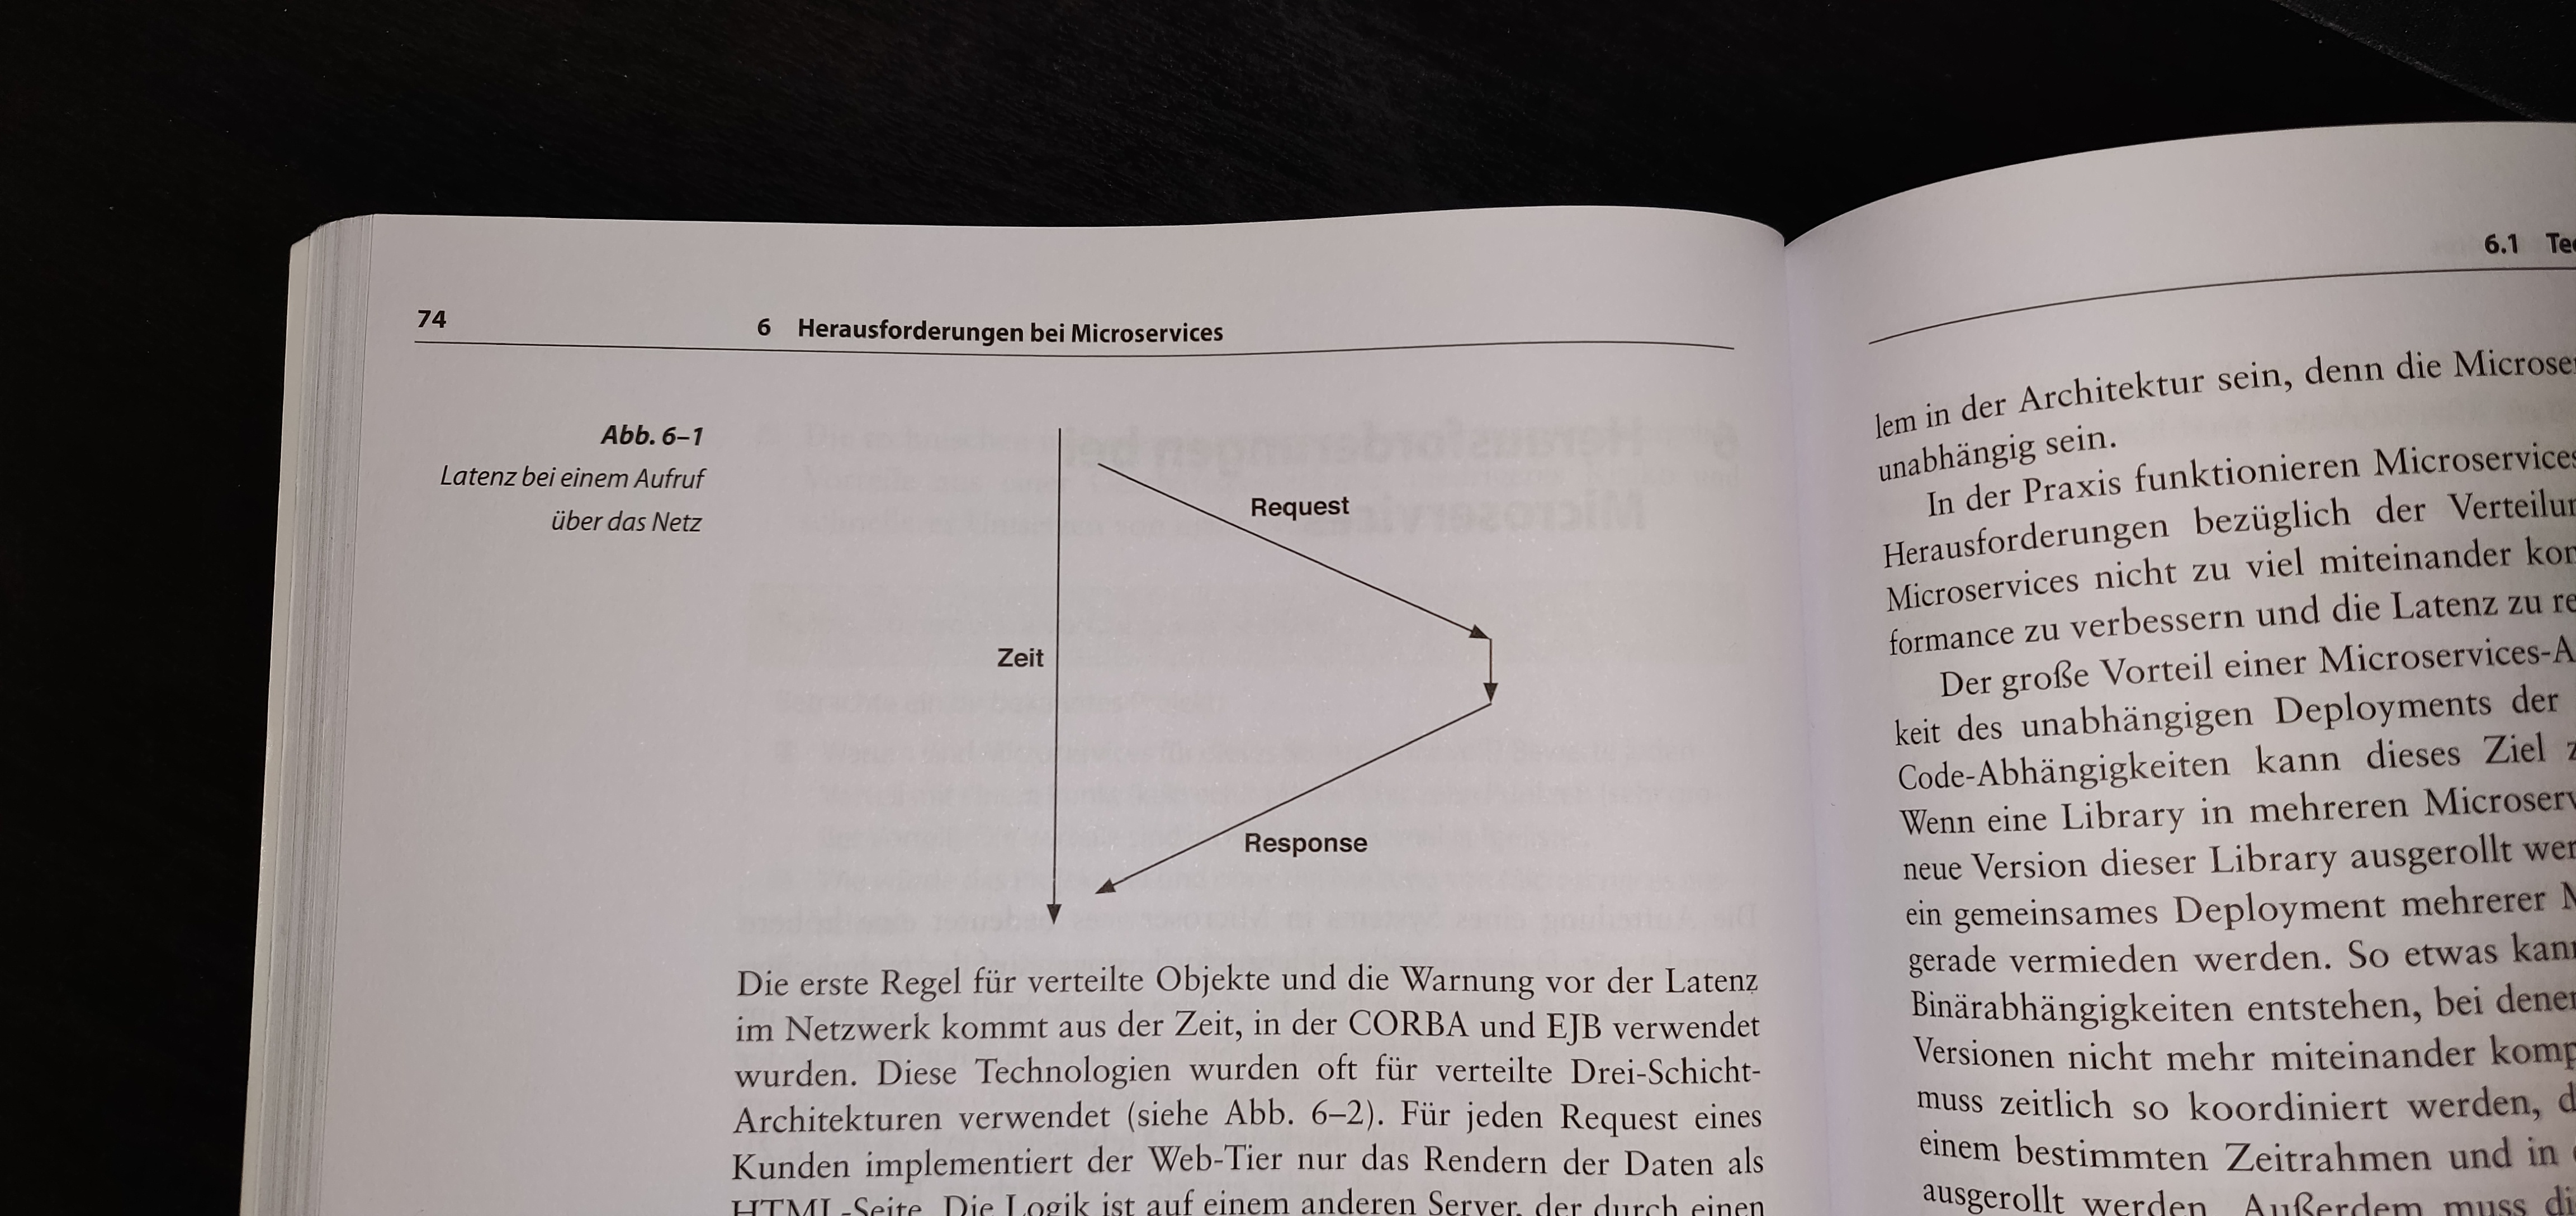
\includegraphics[width=0.7\textwidth]{Graphics/Latenz}
	\caption{Latenz bei einem Netzwerkaufruf}
	\label{fig:Latenz}
\end{figure}

In Fig. \ref{fig:Latenz} ist ein typischer Aufruf über ein Netzwerk zu sehen. Während die Anfrage über das Netzwerk verschickt, von einem anderen Service bearbeitet und die Antwort wieder zurück geschickt wird muss der ursprüngliche Service warten. Selbst wenn die Latenz einer Nachricht nur 0,5 ms beträgt, könnte ein Prozessor mit 3 GHz in dieser Zeit ~1,5 Millionen Operationen durchführen. Daher sollte auf die Entfernung der einzelnen Services geachtet werden und diese so nah wie möglich beieinander zu halten. Auch sollte darauf geachtet werden, dass das Netzwerk nicht überlastet wird. Subnetze bieten sich bei dieser Problemstellung an. \paragraph{}
Eine hohe Kommunikation zwischen Microservices spricht jedoch auch für eine schlechte Skalierung der Services und für zu vielen Abhängigkeiten. Solche Abhängigkeiten sollen jedoch vermeiden werden, da dadurch der Vorteil von Microservices verloren geht - das unabhängige Deployment. Mehr zum Thema Architektur im folgendem Unterkapitel (\ref{ch:Architektur}). \paragraph{}
Ein weiteres Problem welches bei verteilten Systemen auftreten kann, ist der Ausfall eines Teilsystems. Wenn dies geschieht, müssen unterschiedliche Maßnahmen getroffen werden, damit nicht das gesamte System zum Erliegen kommt. So muss es Pläne geben, was passiert, wenn eine Request keine Antwort bekommt. Dafür kann es verschiedene Gründe geben. Es kann beispielsweise daran liegen, dass die Nachricht im Netzwerk nicht richtig weitergeleitet wurde. Eine weitere wahrscheinliche Möglichkeit ist ein abgestürzter Gegenspieler. Im ersten Fall kann durch eine erneut gesendete Anfrage das Problem gelöst werden, im zweiten Fall würde dies jedoch ohne weiteren Maßnahmen zu einer Endlosschleife führen. Dies gilt es zu erkennen und geeignete Fehlerfälle mitzubeachten. \newline
Währenddessen muss der abgestürzte Microservice neu gestartet werden, am Besten wäre es, wenn mehrere Instanzen des Services aktiv wären und im Falle eines Absturzes diese kurzzeitig die zusätzlichen Anfragen bearbeiten könnten. Gleichzeitig wird im Hintergrund der Service automatisch neu gestartet und kann danach weiterarbeiten. \newline
Im Falle von großen Lastwechseln kann dieser Mechanismus auch dazu genutzt werden bei Bedarf neue Instanzen eines Services zu starten, damit keine zu großen Warteschlangen entstehen und die Antwortzeiten gering bleiben. Ein Aufteilen der Requests auf die einzelnen Instanzen kann dabei dann mittels Service Discovery und Load Balancing geschehen.

\section{Architektur} \label{ch:Architektur}
Bei Microservices ist es wichtig, dass die fachliche Struktur mit der Organisationsstruktur übereinstimmt (Gesetz von Conway). Die unterschiedlichen fachlichen Funktionen werden dabei in Microservices aufgeteilt. Ein Team der Organisation ist dabei für einen oder mehrere Microservices zuständig. Die Microservices anderer Teams werden dagegen als Black-Box gesehen, von denen nur die Schnittstelle bekannt ist. Daher können die Microservices auch in unterschiedlichen Technologien implementiert sein. Die einzige Gemeinsamkeit, die alle Services haben müssen, ist eine einheitliche Schnittstelle. Eine valide Option hierfür wäre eine REST Schnittstelle. \newline
Durch die verschiedenen Technologien ist es schwer einen Gesamtüberblick über das System zu behalten. Falls dies jedoch benötigt wird, ist es ratsam einen Technologiestack vorzuschreiben. Dies kann auch partiell durchgeführt werden, falls beispielsweise einheitlich geloggt werden soll. \paragraph{Änderungen}
Durch die Aufteilung in kleine Microservices sind Änderungen und Refactorings innerhalb eines Microservices sehr leicht umzusetzen. Bei größeren Änderungen oder Fehlern ist es auch leicht den gesamten Microservice zu ersetzen und neu zu implementieren. \newline
Falls neue Anforderungen Änderungen an mehreren Microservices erfordern, ist dies sehr viel mehr Arbeit. Kommt dies öfters vor, kann dies auch für eine schlechte Architektur sprechen, die überarbeitet werden sollte. Bei Microservice-übergreifenden Änderungen bei denen mehrere Teams beteiligt sind, müssen diese koordiniert werden und sich miteinander abstimmen. Auch können die Services in unterschiedlichen Technologien entwickelt worden sein oder Bibliotheken in unterschiedlichen Versionen nutzen. Dies alles macht den Vorteil von Microservices zunichte und ist sehr Aufwändig. Daher ist das initiale Erstellen der Architektur ein essentieller Punkt, der über den Erfolg des Projektes maßgeblich mitentscheidet.

\paragraph{Anpassen der Architektur} Wie bereits gezeigt, ist die Architektur ein essentieller Part eines Microservice Systems. Durch eine gute Architektur können Anforderungen nachhaltig schnell umgesetzt werden (Micorservice-intern) und es können die Technologien genutzt werden, die für den Anwendungsfall optimal sind. \newline
Jedoch ändert sich die optimale Architektur mit neuen Anforderungen. Wenn die Architektur daraufhin (agil) angepasst wird, ergibt sich daraus auch kein Problem, jedoch wenn man an der alten Architektur festhält. \newline
Gründe für eine Anpassung der Architektur können folgende sein: \begin{itemize}
	\item Ein Microservice ist zu groß und muss aufgeteilt werden. Zeichen hierfür ist beispielsweise eine schlechte Verständlichkeit oder auch eine Größe, mit der nicht einmal ein ganzes Team zurecht kommt. Ebenfalls kann es vorkommen dass ein Micorservice mehrere Themengebiete umfasst.
	\item Ein Microservice bearbeitet Funktionen, die in einem anderen Microservice besser aufgehoben wären. Erkennbar sind solche Funktionen durch viel Kommunikation zwischen den beiden Services. Ebenfalls können Bereiche in einem Microservice sehr wenig miteinander zu tun haben. Diese können dann aus Gründen der Übersichtlichkeit in neue Microservices getrennt werden.
	\item Wenn eine Funktion von mehreren Microservices genutzt werden soll, sollte eine Architekturänderung ebenfalls in Betracht gezogen werden.
\end{itemize}
Um diese Probleme zu lösen gibt es verschiedene Lösungsansätze: \begin{description}
	\item [Gemeinsame Bibliotheken] Wenn Code gemeinsam genutzt werden soll, so kann dieser in Bibliotheken ausgelagert werden. Dies setzt voraus, dass die darauf zugreifenden Microservices in der selben Technologie entwickelt werden. \newline
	Dies bedeutet jedoch auch, dass die Microservices von einander abhängig werden und die Arbeit an der Bibliothek koordiniert werden muss. \newline
	Durch 3rd. Party Bibliotheken können so ebenfalls Probleme entstehen. So kann in manchen Laufzeitumgebungen jeweils nur eine Version einer Bibliothek genutzt werden. Das heißt, dass wenn in der neuen Bibliothek die externe Bibliothek XY v2.0 benötigt wird, muss der Code des Microservices, wenn er die Bibliothek XY benötigt, diese ebenfalls in der Version 2.0 nutzen. \newline
	Wegen diesen Problemen wird eine Wiederverwendung von Code in Microservices nicht forciert.
	\item [Code übertragen] Ein anderer Weg eine Funktion in einem Microservice verfügbar zu machen, ist die Codeübertragung. Der Ansatz ist wie bei einer gemeinsamen Bibliothek, nur dass keine Abhängigkeiten entstehen. Dadurch kann eine lose Kopplung zwischen zwei Abhängigen und stark kommunizierenden Microservices wiederhergestellt werden. Dabei spielt es keine Rolle ob der Code im ursprünglichem Microservice bestehen bleibt oder nicht, wodurch jedoch Redundanzen entstehen. Dies bedeutet dass Bug Fixes an mehreren Stellen vorgenommen werden müssen, dagegen können sich die Microservices/Funktionen unabhängig voneinander in unterschiedliche Richtungen weiterentwickeln. \newline
	Es muss darauf geachtet werden, dass durch das Hinzufügen von Funktionen der Microservice nicht zu groß wird und zu einem Monolithen mutiert.
	\item[Gemeinsamer Service] Anstatt den Code in eine Bibliothek auszulagern, kann dieser auch in einen neuen Microservice überführt werden. Dadurch werden auch verschiedenen Technologien unterstützt. Mit dieser Methode werden die Micorservices auch klein gehalten, was vorteilhaft für die Übersichtlichkeit und Verständlichkeit des Systems ist. Diese neuen Microservices sind dann reine Backend-Services, da diese keine Benutzeroberfläche besitzen. \newline
	Dieses Verfahren kann auch gut dazu genutzt werden wenn ein Microservice zu groß wird. Durch Auslagern von Funktionen kann die Wartbarkeit wieder erhöht werden.
	\item[Neu schreiben] Mit der Zeit kann es vorkommen dass ein Microservice schwer wartbar wird. Dies kann beispielsweise durch einen ''historisch gewachsenen'' Code geschehen, oder auch durch die Auswahl einer nicht praktikablen Technologie. Gerade bei solchen Problemen haben Microservices ihren Vorteil. \newline
	Durch ihre kleine Größe kann der gesamte Service ohne größeren Aufwand neu entwickelt werden. Dabei können neue Erkenntnisse über die Domäne direkt in die Neuimplementierung einfließen. Ein Wechseln der Technologie ist ebenfalls kein Problem, solang die Schnittstellen gleich bleiben.
\end{description}

\section{Infrastruktur} \label{ch:Infrastruktur}
 Auch bei der Infrastruktur gibt es bei Microservices Hürden und Herausforderungen. So werden viel mehr Server oder Virtuelle Maschinen benötigt als bei einem Monolithen. Die verschiedenen Services müssen aufgrund ihrer Unabhängigkeit auf einzelnen Servern/VM's liegen. Dies kann bspw. an verschiedenen Versionen von Bibliotheken liegen oder auch an dem unabhängigen Deployment der Services. \newline 
Einer der großen Vorteile von Micorservices ist das lastabhängige Starten zusätzlicher Instanzen. Dies muss automatisch und auf einer neuen VM geschehen. Um jedoch überhaupt erstmal festzustellen, wie groß die Last ist, muss ein geeignetes Monitoring auf allen Services aktiv sein. Aufgrund der verschiedenen Technologien kann dies zu einem großen Problem werden. \newline
Ebenfalls sollte ein Monitoring für die Problemfindung vorhanden sein. Dies muss auf die einzelnen Services angepasst sein, damit Schwachstellen erkannt und optimiert werden können. \newline
Auch bei der Entwicklung gibt es im Vergleich zu einem Monolithen Nachteile. So muss für jeden einzelnen Microservice eine Versionskontrolle eingerichtet werden. Eine Build Pipeline pro Micorservice ist ebenfalls empfehlenswert. Diese Entwicklungsanforderungen bedeuten für das Unternehmen zusätzliche Infrastruktur wie auch erhöhte Administration.









\chapter{Daten}\label{ch:Daten}

Die Daten eines Systems, das eine Microservice-Architektur nutzt sind sehr stark verteilt. Dies hat den Grund, das jeder Microservice eine eigene Datenbank besitzt. Würde, wie bei einem Monolithen, alle Daten in einer einzigen Datenbank gespeichert werden, dann würde die Skalierbarkeit sehr stark darunter leiden. Schließlich war einer der Gründe für Microservices, dass jeder der Microservices auf einem eigenen Server laufen könnte, um das System skalieren zu können. Würden alle Daten in einer einzigen Datenbank gespeichert werden (die nur auf einem einzigen Server läuft), würde hier erneut ein Flaschenhals entstehen, da dieser Datenbank-Server nicht im selben Ausmaß skalieren kann, wie es die Microservices können.

Eins der größten Probleme mit den Daten bei einem Microservice-System ist, das durch die Verteilung der Daten keine Transaktionen mehr möglich sind sondern die Änderungen an den Daten anderen Microservices mitgeteilt werden müssen (beispielsweise muss das Anlegen eines Nutzers an andere Microservices mitgeteilt werden).

\section{Synchrone Persistenz}

Synchrone Persistenz ist ein Ansatz um das oben genannte Problem der Synchronisierung zu Lösen. Bei der Synchronen Persistenz wird jede Änderung an den Daten direkt an alle anderen Microservice, die von diesen Daten abhängen, weitergegeben. Wenn beispielsweise ein Microservice B von den Daten des Microservice A abhängt, dann würde B einen Endpunkt besitzen, den A aufruft, sobald sich Daten ändern. A wartet dann auf die Antwort von B, um sicherzustellen, dass die Daten auch tatsächlich in B aktualisiert wurden. Wenn mehrere Microservices von den Daten abhängen, dann muss jeder dieser abhängenden Services einzeln Benachrichtigt werden. Es muss beachtet werden, dass Transaktionen (nach ACID-Prinzip) dennoch nicht möglich sind. Beispielsweise sind Rollbacks nur schwer umsetzbar wenn fünf Microservices Benachrichtigt werden, dies aber nach dem dritten scheitert (es müsste also ein Rollback bei den ersten beiden durchgeführt werden). Desweiteren existieren die folgenden Probleme:

\paragraph{Hohe Kupplung}
Bei der Synchronen Persistenz existiert eine 1:N Beziehung zwischen den Microservices. Das bedeutet, dass im schlechtesten Fall (wenn jeder Microservice immer jeden anderen Microservice benachrichtigen muss) $\dfrac{n(n-1)}{2}$
Beziehungen existieren. Zudem steigt offensichtlich deren Anzahl sehr stark, wenn neue Microservices zum System hinzugefügt werden. Dies erhöht die Komplexität des Systems enorm und macht es für Entwickler sehr schwer, den Überblick zu behalten.

\paragraph{Service-Ausfälle}
Wenn ein einzelner Microservice ausfällt kann dieser nicht mehr Benachrichtigt werden. Hierdurch müsste entweder jeder Microservice speichern, welche Microservices noch Benachrichtigt werden muss (wobei die logik hierfür sehr komplex ist, und den Rahmen eines einzelnen Microservices sprengt), oder der gesamte Befehl scheitert, wodurch allerdings ein Rollback ausgeführt werden müsste, was, wie bereits weiter oben beschrieben, problematisch ist. Zudem würde hierdurch das gesamte System deutlich anfälliger gegenüber Ausfällen werden, da in einem Benachrichtigungs-Baum (d.h. ein Microservice Benachrichtigt andere Microservices, die wiederum andere Microservices benachrichtigen etc.) ein einziger Ausfall eines Microservices den gesamten Baum zum Ausfallen bringt.

\paragraph{Netzwerk-Overhead}
Synchrone Persistenz ist nicht sehr performant, da immer gewartet wird, bis die benachrichtigen Services eine Antwort liefern (da sonst Fehlerbehandlung sehr schwierig wird, da nicht bekannt ist, ob die Services auch tatsächlich benachrichtigt wurden). Wenn hier allerdings ein Baum mit mehreren Ebenen existiert, dann muss der Wurzel-Service warten, bis alle Blatt Services geantwortet haben. Dies kann, je nach Netzwerk-Verbindung oder der Komplexität der Berechnungen bei einer Benachrichtigung, sehr lange dauern.

\section{Ereignis gesteuerte asynchrone Persistenz}

Ereignis gesteuerte asynchrone Persistenz (im folgenden nurnoch Event-Persistenz genannt) ist eine alternative zur Synchronen Persistenz. Der Name beschreibt das Prinzip bereits sehr gut. Es wird ein Ereignis-Basiertes System eingesetzt und, im Gegensatz zur synchronen Persistenz, werden Änderungen nicht sofort, sondern asynchron übernommen. Das bedeutet, dass ein benachrichtigender Microservice nicht auf die Antwort aller benachrichtigten Microservices warten muss, sondern diese möglicherweise erst zu einem späteren Zeitpunkt benachrichtigt werden (hierbei handelt es sich allerdings in der Regel um kleine Zeitverzägerungen, die nicht von einem Menschen bemerkbar ist).
Der Ablauf bei der Event-Persistenz zum Benachrichtigen von anderen Microservices läuft ab, indem der benachrichtigende Microservice, auf einem bestimmten Kanal den Event-Manager benachrichtig, dass es neue Daten gibt. Hierbei existiert ein Kanal, jeweils einer pro möglicher Veränderung (beispielsweise gibt es einen Kanal für das Erstellen und einen Kanal für das Löschen eines Nutzers). Andere Microservices, die benachrichtigt werden müssen, tragen sich beim Event-Manager für einen bestimmten Kanal ein und werden dann automatisch von diesem benachrichtigt, wenn ein neues Event in dem jeweiligen Kanal ausgelöst wurde.
Hierdurch wird die hohe Kupplung der Synchronen Persistenz verhindert, da jeder Microservice immer nur direkt mit dem Event-Manager kommuniziert und nicht von anderen Microservices abhängig ist. Zudem merkt der Event-Manager welche Services bereits benachrichtigt wurden und welche nicht. Wenn also ein einziger Service ausfällt (und demnach nicht benachrichtigt werden konnte), wird dieser lediglich erst später benachrichtigt. Hierdurch bringt ein einziger Ausfall nicht das gesamte System zum Einsturz, wie es bei der Synchronen Persistenz der Fall wäre. Wenn ein Service ausfällt, dann verzögert sich lediglich der Zeitpunkt bei dem der jeweilige Microservice die Datenänderung übernimmt, bis der Service wieder funktionsfähig ist (solche Verzögerungen sind aber ohnehin von vornherein ein Teil des Systems, da es asynchron ist).
Ein großes Problem der Event-Persistenz ist allerdings, dass ein Ausfall des Event-Managers das gesamte System zum erliegen bringt, da dann keine Benachrichtigungen mehr gesendet werden können. Hier muss also dafür gesorgt werden, dass die Ausfallrate des Event-Managers möglichst gering ist. 
Zudem sind Transaktionen, aus den gleichen Gründen wie bereits bei der Synchronen Persistenz, nach wie vor nicht möglich.

\section{2-Phase-Commit}
Das 2-Phase-Commit (2PC) Protokoll ist ein Protokoll, das Transaktionen in einem Verteilten System ausführen kann. Es hat allerdings einige Probleme. Zum einen nutzt es einen Zentralen Manager, der die Transaktionen orchestriert\footnote{Wobei dieses Problem bei der Event-Persistenz ebenfalls existiert.}. Zum anderen ist das Protokoll sehr aufwändig, und hat die Laufzeit $O(n^2)$. Die Geschwindigkeit wird zudem weiterhin von Sperren auf Ressourcen eingeschränkt. Generell wird 2PC nicht bei Microservices verwendet.

\section{Saga}
Sagas\footnote{Saga ist keine Abkürzung, sondern schlicht das normale Wort \glqq Saga\grqq.} sind eine Möglichkeit, mit der sichergestellt werden kann, dass Daten aktualisiert werden, und mit der, bei einem Fehler, diese Änderungen wieder Rückgängig gemacht werden.
Das Prinzip von Sagas ist das folgende:
Jeder Microservice hat für jedes Datum, dass er aktualisieren kann, jeweils eine Funktion $T$ und $C$ (Transaction beziehungsweise Correction). $T$ aktualisiert ein bestimmtes Datum in der lokalen Datenbank des Services. $C$ macht das genaue Gegenteil, indem es eine Aktualisierung rückgängig macht. Für jedes zu aktualisierende Datum existiert eine Saga, die eine Liste von Microservices darstellt. Zum Aktualisieren eines Datums führt der erste Microservice in der Saga seine $T$-Funktion aus. Dannach wird der zweite Service benachrichtigt, der wiederrum seine $T$-Funktion ausführt. Dies wird solange fortgeführt, bis alle Services in der Saga abgearbeitet wurden. Falls während der Durchführung einer $T$-Funktion ein Fehler auftritt kommt die $C$-Funktion zum tragen. Denn anstatt, dass der nächste Service in der Sage benachrichtigt wird, wird der vorangehende benachrichtigt. Dieser wird dann seinen vorangegangenen aufrufen, der dann die $C$-Funktion aufruft und die erneut die gleiche Nachricht an seinen Vorgänger weitergibt. Hierdurch werden sämtliche Daten, die bis zu diesem Zeitpunkt aktualisiert wurden, wieder durch die $C$-Funktionen rückgängig gemacht.
Sagas nutzen ebenfalls einen Event-Manager, um die Benachrichtigungen zwischen den Services in einer Saga zu verwalten. Hierdurch wird das gesamte System asynchron, und Ausfälle einzelner System sind weniger schwerwiegend.
Die Reihenfolge, in der die Microservices in einer Saga auftreten, muss spezifisch für jede Saga festgelegt werden, hier gibt es keine einheitliche Regel.
Ein Nachteil von Sagas ist, dass sie nicht so lose gekuppelt sind wie es bei der Event-Persistenz der Fall ist. Schließlich müssen bei einer Saga immer alle Services, die Teil dieser Saga sind, gespeichert werden. Vor allem müssen diese im vornherein gut geplant sein, um festzulegen, wie die Reihenfolge der Services innerhalb der Saga auszusehen haben.

\chapter{Fallstudie}\label{ch:Fallstudie}
\paragraph{Szenario}
Für unseren Online-Shop soll eine neue Benutzerverwaltung entwickelt werden, nachdem die alte nicht mehr Wartbar ist. Dazu zählt das Anmelden und neu registrieren von Nutzern wie auch das ausgeben der Benutzerdaten.

\paragraph{Gründe für einen Microservice}
Da man aus den Problemen der Vorherigen Benutzerverwaltung lernt, soll die neue Verwaltung auch langfristig Wartbar bleiben. \newline
Auch soll jedes Teilgebiet der Anwendung von einem einzelnen Team umgesetzt werden.
\chapter{Fazit}

Letztendlich erreicht die Microservice Architektur ihr Ziel: Systeme können sehr gut auf viele Server verteilt und damit skaliert werden. Allerdings ist die Architektur nicht in jeder Situation optional, denn für jeden Vorteil, den die Architektur gegenüber der klassischen Monolith Architektur hat, existiert ein Nachteil, der andere Probleme macht. Beispielsweise sind die Daten zwar sehr verteilt, dafür ist es allerdings deutlich schwerer die Daten als Ganzes zu verwalten und Transaktionen sind praktisch nur sehr schwer umsetzbar. Letztendlich bleibt jedoch der Vorteil der Skalierbarkeit bestehen und wenn bei einem großem System die Wahl zwischen den skalierenden Microservices und einem nicht skalierendem Monolithen besteht, dann müssen selbstverständlich die Microservices gewählt werden, da das System sonst schlicht nicht umsetzbar ist. Ein Monolith ist allerdings eine völlig valide und gerechtfertigte Wahl, wenn die Skalierbarkeit eines Microservice-Systems nicht benötigt wird.

%\cleardoublepage\include{Chapters/KapitelBachelorarbeit} % <<< Hier alle Chapter der Abschlussarbeit (einzeln) einbinden

%********************************************************************
% Bibliography/References
%*******************************************************
\cleardoublepage%********************************************************************
% Bibliography
%*******************************************************
\printbibliography

%********************************************************************
% List of Figures etc.
%*******************************************************
\cleardoublepage%*******************************************************
% Verzeichnisse (Abbildungen, Tabellen, Listings, etc.)
%*******************************************************
\cleardoublepage
\begingroup
	\let\clearpage\relax
	\let\cleardoublepage\relax
	\listoffigures
	%\listoftables
	%\addcontentsline{toc}{chapter}{\lstlistlistingname}
	%\lstlistoflistings 
\endgroup 
%*******************************************************
% Abkürzungsverzeichnis
%*******************************************************
\chapter*{Abkürzungsverzeichnis}
\addcontentsline{toc}{chapter}{Abkürzungsverzeichnis}	
	%Hier alle benötigten Abkürzungen einfügen
	\begin{acronym}[WLAN] % LONGEST ACRONYM HERE FOR CORRECT SPACING
	    \acro{WLAN}{Wireless Local Area Network}
	    \acro{TCP}{Transmission Control Protocol}
	    \acro{GoF}{Gang of Four}
	\end{acronym}
	
	

% ********************************************************************
% Appendix/Anhang
%***************************************************************
\appendix
\part*{Anhang}
\cleardoublepage%********************************************************************
% Appendix
%*******************************************************
\chapter{Erster Abschnitt des Anhangs}
In den Anhang gehören "`Hintergrundinformationen"', also weiterführende Information, ausführliche Listings, Graphen, Diagramme oder Tabellen, die den Haupttext mit detaillierten Informationen ergänzen. 

\blindtext
\blindtext
\blindtext



%*******************************************************
\cleardoublepage\pagestyle{empty}

\hfill

\vfill


\pdfbookmark[0]{Kolophon}{colophon}
\section*{Kolophon}
Dieses Dokument wurde mit der \LaTeX-Vorlage für Abschlussarbeiten an der htw saar im Bereich Informatik/Mechatronik-Sensortechnik erstellt (\currentVersion). Die Vorlage wurde von Yves Hary und Andr\'e Miede entwickelt (mit freundlicher Unterstützung von Thomas Kretschmer, Helmut G. Folz und Martina Lehser). Daten: (F)\makeatletter\f@size\makeatother\ -- (B)\the\textwidth\ -- (H)\the\textheight\ 


\end{document}
% ********************************************************************
